%% Document created 27 November 2021 automatically 
%% from /Users/massimosotgia/Desktop/uni_at_DIFI/Lab2/setup.py 

%% Copyright (C) Mattia Sotgia et al. 2022
%% Using class revtex4-2.cls

\documentclass[
    rmp,
    % preprint,
    % linenumbers,
    % tightlines,
    reprint, 
    superscriptaddress, 
    altaffilletter, 
    amsmath, 
    amssymb,
    a4paper]{revtex4-2}

\usepackage[top=1.75cm,bottom=2.5cm,left=1.5cm,right=1.5cm]{geometry}

\usepackage[utf8]{inputenc}
\usepackage[T1]{fontenc}

\usepackage[italian]{babel}

%% revtex4-2 bug-fix
\def\andname{e}
%--------------------
\makeatletter
\let\it@comma@def\active@comma
\makeatother

\usepackage{txfonts}
\usepackage{graphicx}% Include figure files
\graphicspath{{../fig/}}

\usepackage{dcolumn}% Align table columns on decimal point
\usepackage{bm}% bold math
\usepackage[colorlinks, urlcolor=., bookmarks]{hyperref}% add hypertext capabilities
\renewcommand\UrlFont{\color{blue}}

\usepackage{physics}
\usepackage{siunitx}

\usepackage{fancyhdr}
\pagestyle{fancy}
\fancyhf{}
\def\twodigits#1{\ifnum#1<10 0\fi\the#1}

%-----------------------------------------------------------------------------------------------

\usepackage{background}
\SetBgColor{gray}
\SetBgAngle{90}
\SetBgScale{2}
\SetBgVshift{0.27\textwidth}

\usepackage[american resistors]{circuitikz}
\usepackage{listings}
\lstset{
  basicstyle=\fontsize{5}{6}\selectfont\ttfamily,
  % backgroundcolor=\color{white},   % choose the background color
  % basicstyle=\footnotesize,        % the size of the fonts that are used for the code
  breakatwhitespace=false,         % sets if automatic breaks should only happen at whitespace
  breaklines=true,                 % sets automatic line breaking
  captionpos=b,                    % sets the caption-position to bottom
  % commentstyle=\color{mygreen},    % comment style
  deletekeywords={...},            % if you want to delete keywords from the given language
  escapeinside={\%*}{*)},          % if you want to add LaTeX within your code
  % extendedchars=true,              % lets you use non-ASCII characters; for 8-bits encodings only, does not work with UTF-8
  % firstnumber=1000,                % start line enumeration with line 1000
  % frame=single,                    % adds a frame around the code
  % keepspaces=true,                 % keeps spaces in text, useful for keeping indentation of code (possibly needs columns=flexible). 
  % keywordstyle=\color{blue},       % keyword style
  % numbers=left,                    % where to put the line-numbers; possible values are (none, left, right)
  % numbersep=5pt,                   % how far the line-numbers are from the code
  numberstyle=\tiny\color{gray}, % the style that is used for the line-numbers
  % rulecolor=\color{black},         % if not set, the frame-color may be changed on line-breaks within not-black text (e.g. comments (green here))
  showspaces=false,                % show spaces everywhere adding particular underscores; it overrides 'showstringspaces'
  showstringspaces=false,          % underline spaces within strings only
  showtabs=false,                  % show tabs within strings adding particular underscores
  stepnumber=2,                    % the step between two line-numbers. If it's 1, each line will be numbered
  % stringstyle=\color{mymauve},     % string literal style
  tabsize=2,                       % sets default tabsize to 2 spaces
}
\usepackage{soul}


%% Define ref types
\newcommand{\reftab}[1]{Tabella {\ref{#1}}}%
\newcommand{\reffig}[1]{Figura {\ref{#1}}}%
\newcommand{\refeqn}[1]{({\ref{#1}})}%
\newcommand{\ChiSqr}{$\chi^2$\space}
\newcommand{\ChiNdf}{$\chi^2/\text{ndf}$}
\newcommand{\cernroot}{\texttt{root}}
\newcommand{\treSigma}{$3\sigma$}
\newcommand{\stdErr}[1]{$\varepsilon_{#1}$}
\newcommand{\mstdErr}[1]{\varepsilon_{#1}}
%% PAPER ONLY custom Macros

\newenvironment{methods}[1]{\section*{#1}
%\fontfamily{phv}
\fontsize{7.5}{9}\selectfont\label{sec:methods}\noindent}{\par\noindent}

%\usepackage{lcsec}

\sisetup{
    % separate-uncertainty=true,
    round-mode=uncertainty,
    % exponent-mode = scientific
}

\fancyfoot[C]{
    \the\year\twodigits\month\twodigits\day/4-\thepage
}
\fancyhead[C]{\fontfamily{phv}\fontsize{12}{12}\selectfont RELAZIONE DI LABORATORIO \textbf{
    N. 2 % ! <== CAMBIARE (Nessuna rel. -> 00)
    } (\the\year)
}

\newcommand{\LMopamp}{{\fontfamily{phv}\selectfont\small\bf LM741}}

\begin{document}

\title{Verifica sperimentale della dipendenza quadratica inversa $d^{-2}$ del calore irradiato rispetto distanza 
}
\thanks{Esperienza n. 4
}

\author{Francesco Polleri}
\email{s5025011@studenti.unige.it}
\author{Mattia Sotgia}
\email{s4942225@studenti.unige.it}

\collaboration{Gruppo A1}
\affiliation{Dipartimento di Fisica, Università degli Studi di Genova}

\date{presa dati
    30 novembre, 1-2 dicembre 2021, consegnata in data 
    \today
}

\begin{abstract}
    
\end{abstract}
\maketitle
\thispagestyle{fancy}
% Rimuovere per consegna
\SetBgContents{
    laboratorio2: e4 (non per la consegna) \today % ! Note di versione
}

%%%% CORPO DEL TESTO
%%%% CORPO DEL TESTO

\section*{Introduzione}
Lo scopo principale di questa esperienza di laboratorio è fare una verifica sperimentale della dipendenza quadratica inversa dell'energia irradiata da una sorgente luminosa in funzione della distanza da essa.
Per fare le misure necessarie abbiamo bisogno di diversi dispositivi e in particolare sfrutteremo il funzionamento di amplificatori per strumentazione, basati su amplificatori operazionali.

Come sorgente luminosa usiamo una piccola lampadina ad incandescenza che possiamo posizionare a diverse distanze da un termometro al platino (PT100) che usiamo quindi come sensore e la cui caratteristica principale è la dipendenza lineare, a temperature intorno a quella ambiente, della resistenza in funzione della variazione di temperatura (la derivata è \SI{0.4}{\ohm/\kelvin}). 

% \hl{Poich\'e vogliamo misurare delle variazioni di temperatura attraverso la variazione del valore di una resistenza, utilizziamo un ponte di Wheatstone in modo che le nostre misure siano il pi\`u precise possibili e per vedere ancora meglio gli effetti di queste variazioni sulla nostra uscita del segnale usiamo un amplificatore per strumentazione.}

\section*{Studio e caratterizzazione di un amplificatore operazionale}
\label{sec:studio_caratt_op_amp}

Poiché l'amplificatore per strumentazione che utilizziamo per la nostra misura è costituito da tre amplificatori operazionali inseriti in un unico circuito, ci interessa studiare meglio il loro comportamento in modo da progettare il circuito nel modo migliore possibile.

\begin{figure}[b!]
    \begin{circuitikz}
        \draw (0,0)
        node[op amp, scale=0.5] (opamp) {}
        (opamp.-) to [short, -*] (-1, 0.25)
        to [R=$R_{1}$, resistors/scale=0.8] node[left]{in}(-2.5, 0.25)
        (-1, 0.25) -- (-1, 1) to [R=$R_{2}$, resistors/scale=0.8](1, 1)
        to [short, -*] (1, 0)
        (opamp.out) -- (2,0) node[right]{out}(2, 0)
        (opamp.+) -- (-1, -0.25) -- (-1, -0.75) node[ground]{}
        ;
    \end{circuitikz}
    \caption{Schema circuitale amplificatore invertente}
    \label{fig:amp_inv}
\end{figure}

Iniziamo costruendo un semplice circuito (\reffig{fig:amp_inv}) con un amplificatore LM741 alimentato con $\pm V_{cc}=\pm \SI{15}{\volt}$ e progettato in modo che il guadagno ad anello chiuso sia $G_{\text{close}}=80$. Attraverso lo studio del circuito troviamo che il guadagno risulta essere $G=-R_{1}/R_{2}$. Per scegliere le resistenze da inserire nel circuito non ci basiamo però solo su questa condizione, bensì le prendiamo in modo che siano molto più grandi della resistenza interna del generatore che dovrebbe essere circa \SI{50}{\ohm}. Prendiamo quindi come valore nominale di $R_{1}$ \SI{1}{\kilo\ohm}, mentre per $R_2$ \SI{80}{\kilo\ohm}. Misuriamo le resistenze con il tester a nostra disposizione e troviamo che $R_{1}=\SI{0.988 +- 0.006}{\kilo\ohm}$ mentre $R_{2}=\SI{82.7 +- 0.5}{\kilo\ohm}$ 

Per effettuare la misura del guadagno raccogliamo 5 valori della tensione di uscita ($V_{out}$) con i rispettivi valori della tensione di entrata ($V_{in}$) a \SI{50}{\hertz} (\reffig{fig:guadagno_inv_noninv}, configurazione invertente) in modo da acquisire i dati in una zona in cui il guadagno non dipende dalla frequenza poiché l'amplificatore si comporta come un passa basso. Inoltre i valori di $V_{in}$ li abbiamo scelti in modo che, una volta amplificati, fossero comunque minori di \SI{15}{\volt}, che è la tensione con cui alimentiamo l'amplificatore, perché altrimenti il valore di $V_{out}$ sarebbe appunto uguale a $V_{cc}$. Eseguendo un fit lineare usando come funzione \[V_{out}=G\cdot V_{in}+q\] e impostando come parametri $G$ e $q$ otteniamo quindi che 
\begin{align*}
    G & =\num{78.6454 +- 8.1} \\
    q & =\SI{0.03}{\volt} \\ 
\end{align*}

Osserviamo quindi che il valore di $G$ è compatibile con il valore che volevamo ottenere, cioè $G=80$ e che la quota della retta è compatibile con zero e ciò rispecchia il fatto che se la tensione in entrata è nulla, anche quella in uscita deve esserlo.

Utilizzando sempre lo stesso circuito vogliamo creare un diagramma di Bode della funzione di trasferimento, in modo da osservare effettivamente il comportamento da passa-basso e da trovare la frequenza di taglio. Impostiamo quindi la $V_{in}$ a \SI{100}{\milli\volt} e raccogliamo i valori di $V_{in}$, $V_{out}$ e del periodo $T$ con i loro rispettivi fondo scala, facendo variare la frequenza da \SI{100}{\hertz} fino \SI{20}{\kilo\hertz} raccogliendo circa 3 punti per ogni decade. Realizziamo un fit sui dati usando come funzione  \begin{equation}\left|H[\nu]\right|=\frac{G}{\sqrt{1+\left(\frac{\nu}{\nu_0}\right)^2}} \label{eq:H}\end{equation} e scegliendo come parametri $G$ e $\nu_0$. 
Otteniamo quindi che
\begin{align*}
    G     &=\num{ 83.2458 +- 1.24581} \\
    \nu_0 &=\SI{8.71835 +- 0.2559}{\kilo\hertz} \\ 
\end{align*}

Ripetiamo lo stesso procedimento utilizzando però come $R_2$ una resistenza da \SI{8}{\kilo\ohm} in modo che il guadagno sia 10 volte più piccolo. Vogliamo quindi verificare che il prodotto $\nu_0 \cdot G $ è costante. Raccogliamo quindi i nuovi dati e realizziamo un altro fit usando di nuovo l'equazione \refeqn{eq:H} e impostando gli stessi parametri e troviamo che
\begin{align*}
    G     &=\num{7.99818 +- 0.101188} \\
    \nu_0 &=\SI{85.4452 +- 2.31586}{\kilo\hertz} \\ 
\end{align*}
Osserviamo che effettivamente il guadagno si presenta essere circa 10 volte più grande del valore misurato in precedenza.

Nel primo caso il prodotto vale \num{68.3406 +- 2.04412e4}, mentre nell'altro caso vale \num{72.5766 +- 2.39117e4} e troviamo che quindi sono effettivamente compatibili.

\begin{figure}
    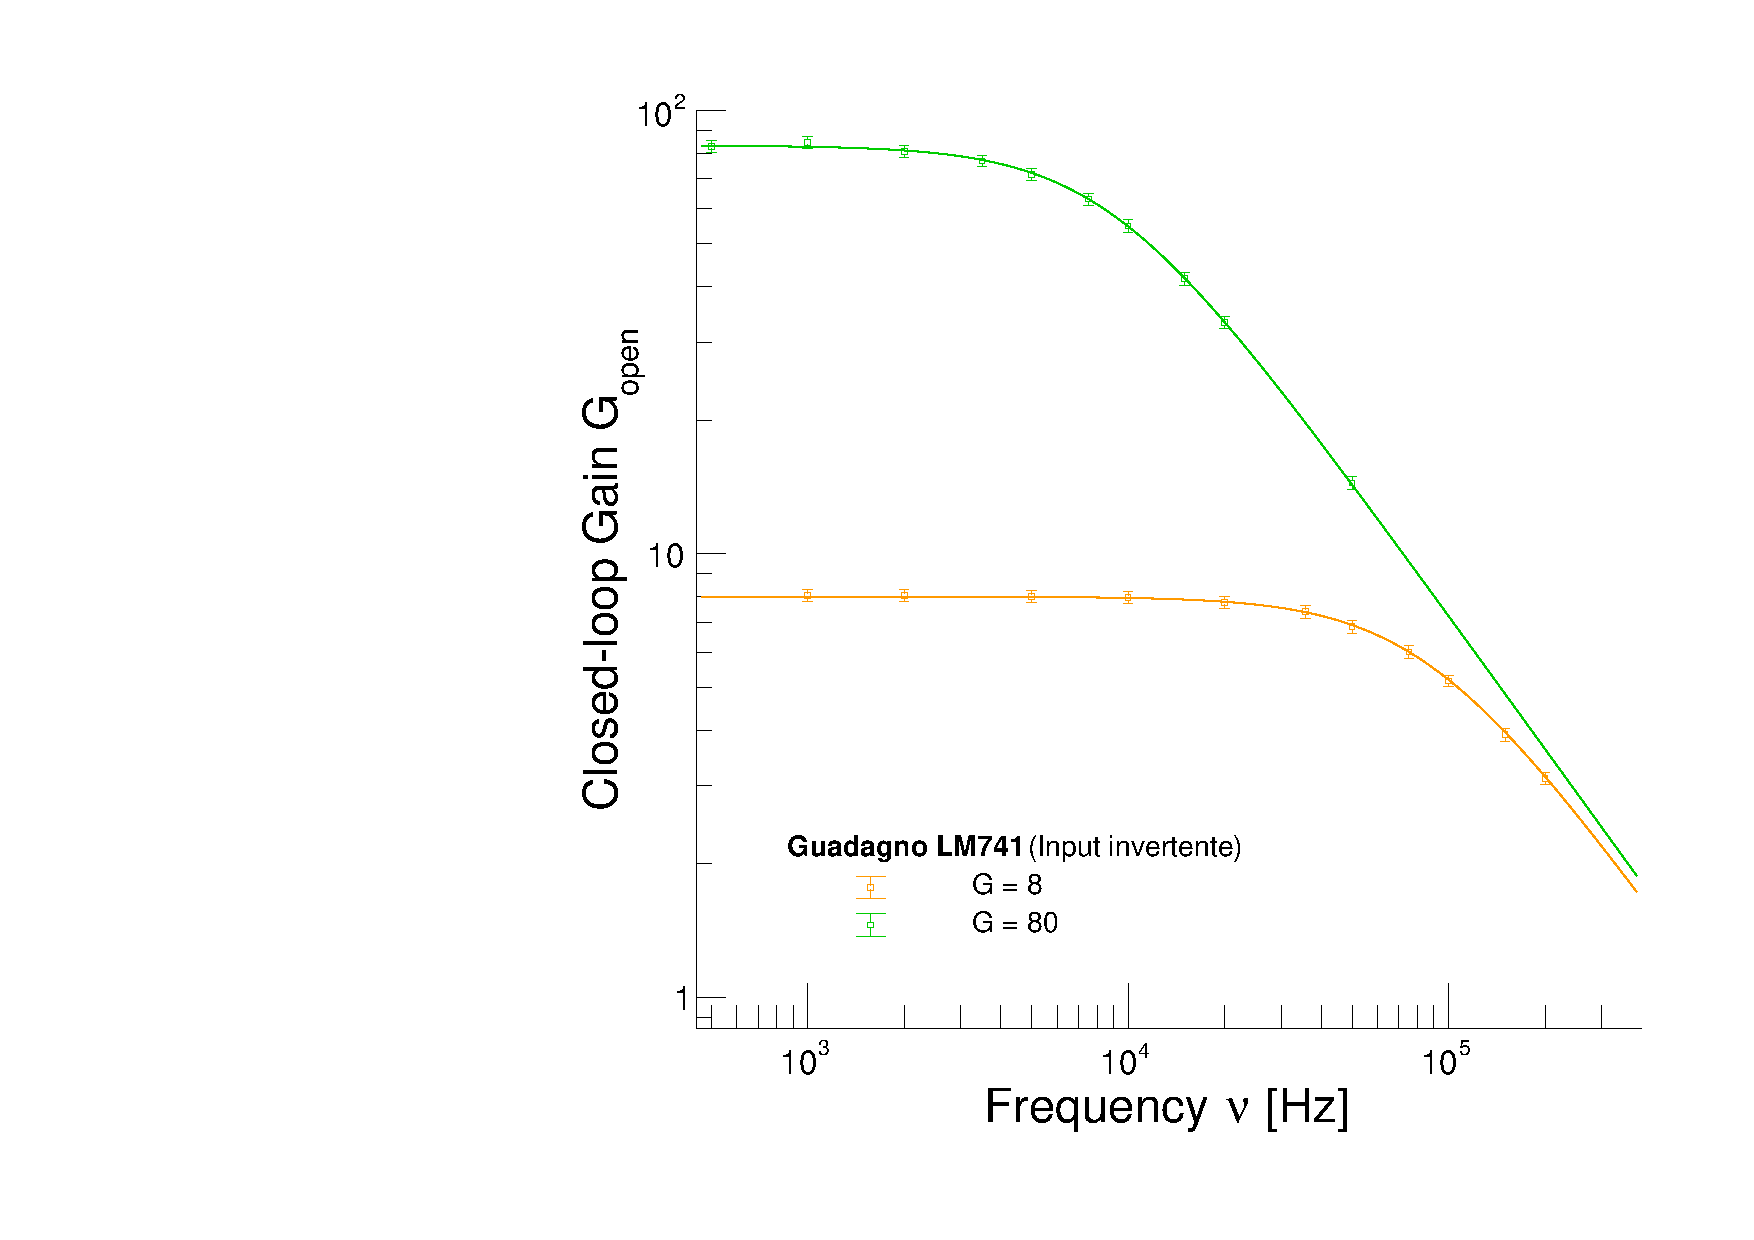
\includegraphics[width=\linewidth]{plot_combined.pdf}
    \caption{Grafico combinato dei diagrammi di Bode dell'amplificatore operazionale LM741 ottenuti in differenti configurazioni invertenti tali da avere guadagni diversi, ma possiamo osservare che convergendo asintoticamente sul fronte di discesa, possiamo qualitativamente verificare la conservazione del GBW (\emph{Gain-Bandwidth}).}
    \label{fig:plot_combined}
\end{figure}

Inoltre dalla \reffig{fig:plot_combined} possiamo osservare anche visualmente che il prodotto che prima abbiamo quantitativamente verificato essere costante sia visibile anche sovrapponendo i due diagrammi. Infatti possiamo osservare che diminuendo il guadagno $G_{\text{close}}$ da 80 a 8, ovvero cambiando $R_1$ da \SI{80}{\kilo\ohm} a \SI{8}{\kilo\ohm}, osserviamo che la frequenza di taglio si sposta di un fattore 10, passando da \SI{8}{\kilo\hertz} a \SI{80}{\kilo\hertz}.

Un'altra cosa che vogliamo misurare è il valore dell'impedenza di ingresso per verificare che come da modello sia effettivamente pari ad $R_1$. Per fare questo colleghiamo in serie una resistenza che abbia lo stesso valore di $R_1$ tra il punto che porta $V_{in}$ e $R_1$. Misuriamo quindi la tensione in uscita nel nodo di congiunzione tra le due resistenze e troviamo che il valore di $V_{out}$ è circa pari a $\frac{V_{in}}{2}$ e ciò significa che la tensione si è ripartita a metà tra la nuova resistenza che abbiamo inserito e l'impedenza di ingresso del circuito e quindi effettivamente l'impedenza di ingresso del nostro circuito è proprio $R_1$.

\begin{figure}[t!]
    \begin{circuitikz}
        \draw (0,0)
        node[op amp, scale=0.5, yscale=-1] (opamp) {}
        (opamp.-) -- (-1, -0.25) to [short, -*] (-1, -1)
        to [R=$R_{1}$, resistors/scale=0.8] node[ground]{}(-1, -2.5)
        (-1, -0.25) -- (-1, -1) to [R=$R_{2}$, resistors/scale=0.8](1, -1)
        to [short, -*] (1, 0)
        (opamp.out) -- (2,0) node[right]{out}(2, 0)
        (opamp.+) -- (-1, 0.25) node[left]{in}
        ;
    \end{circuitikz}
    \caption{Schema circuitale amplificatore non-invertente}
    \label{fig:amp_noninv}
\end{figure}

Successivamente costruiamo un circuito amplificatore non-invertente il cui schema è riportato in \reffig{fig:amp_noninv} e utilizzando le stesse resistenze usate in precedenza. Ripetiamo quindi gli stessi procedimenti fatti prima per trovare il guadagno (\reffig{fig:guadagno_inv_noninv}, configurazione non-invertente) e troviamo che
\begin{align*}
    G &=\num{81.5167+-7.03287} \\
    q &=\SI{0.180687+-0.818311}{\volt} \\ 
\end{align*}

per cui il guadagno è compatibile con quello che avremmo dovuto ottenere da modello cioè $G=1+R_1/R_2$ mentre la quota è compatibile con zero.

Per misurare la tensione di ingresso del circuito ripetiamo ciò che avevamo fatto prima e questa volta troviamo che $V_{out}$ è praticamente uguale a  $V_{in}$. Ciò significa che la resistenza di ingresso del circuito è molto più grande di \SI{1}{\kilo\ohm} perché infatti sulla nuova resistenza inserita non vi è praticamente caduta di potenziale. Ciò significa che il modello è verificato in quanto la resistenza di ingresso dovrebbe essere infinita, cioè realisticamente nell'ordine di \SI{1}{\mega\ohm}.

Un'altra caratteristica dell'amplificatore che possiamo misurare è la cosiddetta \emph{slew rate}. La \emph{slew rate} è una grandezza che indica la velocità, espressa in volt su secondi, con cui un dispositivo o circuito elettronico è capace di reagire, sollecitato sul suo ingresso, da un impulso di tensione, il cui valore, da minimo a massimo, è contenuto in un tempo brevissimo. Per misurarla costruiamo un comparatore a soglia nulla, il cui schema è riportato in \reffig{fig:opamp_comparatore} e mandiamo in ingresso un'onda quadra. Poiché quindi la risposta del circuito non è immediata, sull'oscilloscopio non osserviamo un'onda quadra, bensì dei trapezi isosceli e ciò che a noi interessa è proprio la pendenza dei lati obliqui di questi trapezi. Utilizzando i cursori dell'oscilloscopio possiamo quindi misurare il rapporto tra la variazione di tensione ($\Delta Y$) e l'intervallo di tempo ($\Delta X$). Troviamo quindi che il valore dello slew rate è \SI{0.54076305 +- 0.016294305}{\volt\per\micro\second} che è molto vicino al valore indicato sul data-sheet del dispositivo.

\begin{figure}
    \begin{circuitikz}
        \draw (0,0)
        node[op amp, noinv input up, scale=0.75](opamp){\texttt{LM741}}
        (opamp.+) -- (-2, 0.375) node[left]{in}
        (opamp.-) -- (-2, -0.375) -- (-2, -0.75) node[ground]{}
        (opamp.out) -- (1, 0) node[right]{out}
        (opamp.up) -- ++(0, 1) node[above]{+Vcc}
        (opamp.down) -- ++(0, -1) node[below]{-Vcc}
        ;
    \end{circuitikz}
    \caption{Schema circuitale del comparatore utilizzato per effettuare la misura della \emph{slew rate}.}
    \label{fig:opamp_comparatore}
\end{figure}

\section*{Studio e caratterizzazione amplificatore per strumentazione}
Vogliamo costruire un amplificatore per strumentazione a due stadi il cui guadagno sia compreso tra 100 e 200. Infatti avere un guadagno troppo alto porta il segnale di uscita ad essere troppo sensibile a rumori e fluttuazioni. Dallo studio del circuito riportato in \reffig{fig:circ:strum_amp} troviamo che se $R_{b}=R_{b}'$, $R_{c}=R_{c}'$ e $R_{d}=R_{d}'$ il guadagno è dato da \[G=\frac{R_{d}}{R_{c}}\cdot \left(1+2\cdot \frac{R_{b}}{R_{a}}\right).\] 

Prendiamo quindi come resistenze:
\begin{align*}
    R_a &= \SI{17.8 +- 0.11}{\kilo\ohm}\\
    R_b &= \SI{37.5 +- 0.166}{\kilo\ohm}\\
    R_c &= \SI{1.0 +- 0.064}{\kilo\ohm}\\
    R_d &= \SI{32.2 +- 0.151}{\kilo\ohm}\\
    R_b'&= \SI{37.5 +- 0.166}{\kilo\ohm}\\
    R_c'&= \SI{1.0 +- 0.064}{\kilo\ohm}\\
    R_d'&= \SI{32.2 +- 0.151}{\kilo\ohm}\\
\end{align*}
(Per assicurarci che le resistenze che volevamo fossero uguali, avessero lo stesso valore abbiamo misurato ogni resistenza con il tester).
Il valore del guadagno dovrebbe quindi essere \num{1.68 +- 0.12e2}. 

\begin{figure}
    \begin{circuitikz}
        \circuitikzset{resistors/scale=0.4}
        \draw 
        (0,0) node[op amp, noinv input up, scale=0.5, anchor=-](OA1){\texttt{LF356}}
        (OA1.+) -- ++(-1, 0) node[above]{{\tiny \texttt{Non inverting input}}}
        (0,-3) node[op amp, scale=0.5, anchor=-](OA2){\texttt{LF356}}
        (OA2.+) -- ++(-1, 0) node[above]{{\tiny \texttt{Inverting input}}}
        (OA1.-) to [short, -.] (0,-0.75) to [R=$R_a$] (0,-2.25)
        (OA2.-) to [short, -.] (0, -2.25) to [R=$R_b$] (1.5, -2.25) -. (1.5, -3.25)
        (0, -0.75) to [R=$R_b'$](1.5, -0.75) -. (1.5, 0.25)
        (OA1.out) -- (1.5, 0.25) to [R=$R_c'$] (2.5, 0.25) -- ++(0.5, 0) -- (3, -1.5) 
        (2.5, -1) node[ground]{} to [R=$R_d'$] (2.5, 0.25) 
        (OA2.out) -- (1.5, -3.25) to [R=$R_c$] (3, -3.25) -- (3, -2)
        (3, -2) node[op amp, noinv input up, scale=0.5, anchor=-](OAout){\texttt{LF356}}
        (OAout.out) -- ++(1, 0) node[above]{\texttt{\tiny Out}}
        (3, -3.25) to [R=$R_d$] (4.5, -3.25) -- (4.5, -1.75)
        ;
    \end{circuitikz}
    \caption{Schema circuitale amplificatore per strumentazione.}
    \label{fig:circ:strum_amp}
\end{figure}

Il circuito integrato nell'amplificatore per strumentazione (Figure \ref{fig:circ:strum_amp} e \ref{fig:circ_all}) è caratterizzato da un guadagno complessivo dato da \begin{equation}V_{out} = G_{\text{diff}}\cdot \left(V_{\text{non-inv}}-V_{\text{inv}}\right) +  G_{\text{CM}}\cdot V_{\text{CM}} + V_{\text{offset}}.\label{eq:V_out=GtotVin}\end{equation}
$V_{\text{offset}}$ è il valore di offset dello strumento, ovvero il valore $V_{out}$ che troviamo anche in assenza di segnale di ingresso $\left(V_{\text{non-inv}}-V_{\text{inv}}\right)$ ed è causato dalla presenta di una differenza reale dei due amplificatori che usiamo nel primo stadio e di conseguenza anche nelle correnti che scorrono in essi.\\
$G_{\text{CM}}$ è invece il guadagno di modo comune che è presente poiché le resistenze scelte $R_c/R_d$ e $R_c'/R_d'$ non sono coppie uguali perfettamente, e rendono asimmetrico l'ingresso, introducendo una tensione di modo comune $V_{\text{CM}}$ che è la media delle tensioni in ingresso.\\
$G_{\text{diff}}$ è il guadagno differenziale e caratterizza il guadagno ideale che il circuito dovrebbe avere se i segnali in ingresso sono simmetrici rispetto allo zero, rendendo il termine $G_{\text{CM}}\cdot V_{\text{CM}} = 0$. 

Per misurare il valore di offset vogliamo quindi che i primi due termini di \refeqn{eq:V_out=GtotVin} vengano annullati. Poniamo dunque \[V_{\text{non-inv}}=V_{\text{inv}}=0\] e osserviamo il valore della tensione in uscita, verificando dove si pone la tensione in uscita $V_{out}$ rispetto al valore di terra.
Possiamo quindi usare un \emph{trimmer} presente sulla scheda in modo da modificare la corrente in ingresso e cercare di eliminare l'offset.

Posto l'offset ad un valore trascurabile (nell'ordine dei \unit{\milli\volt}), procediamo a valutare il valore di $G_{\text{CM}}$ ponendo \[V_{\text{non-inv}}=V_{\text{inv}}\neq0\]
ed effettuando 5 diverse misure del valore di $V_{out}$ per 5 diversi valori di $V_{in}$ (\reffig{fig:guadagno_op_amp_strum}, sopra) e facendo quindi un fit secondo l'equazione $V_{out}=G_{\text{CM}}\cdot V_{in}+q$ scegliendo come parametri $G_{\text{CM}}$ e $q$. Troviamo quindi che i valori dei parametri sono rispettivamente
\begin{align*}
    G_{\text{CM}} &=\num{0.0132857+-0.00105784} \\
    q &=\SI{0.172163+-0.099093e-2}{\volt} \\
\end{align*}
e notiamo che giustamente il valore della quota è compatibile con zero.

Misurato il $G_{\text{CM}}$, procediamo a calcolare il valore di $G_{\text{diff}}$ (\reffig{fig:guadagno_op_amp_strum}, sotto) usando lo stesso metodo con cui abbiamo trovato $G_{\text{CM}}$ senza però impostare $V_{\text{non-inv}}=V_{\text{inv}}$. I valori dei parametri che il fit ci restituisce sono
\begin{align*}
    G_{\text{diff}} &=\num[round-mode=none]{183+-16} \\
    q &=\SI{-0.044431+-0.449922}{\volt} \\
\end{align*}
La quota è compatibile con zero e il valore di $G_{\text{diff}}$ è compatibile con il guadagno teorico che avevamo calcolato quando abbiamo scelto le resistenze da inserire nel circuito ($G_{\text{teorico}}=$\num{1.68 +- 0.12e2}). Inoltre vediamo anche che $G_{\text{diff}}$ è diversi ordini di grandezza più grande di $G_{\text{CM}}$ per cui possiamo considerare quest'ultimo trascurabile. Infatti il rapporto di reiezione di modo comune (CMRR) è pari a \num{13.777+-1.6063e3}.

Un altra caratteristica che possiamo misurare è la banda passante dell'amplificatore. Per fare ciò impostiamo la tensione di ingresso a diverse frequenze e raccogliamo i valori di $V_{out}$ per costruire un diagramma di Bode della funzione di trasferimento e calcolare la frequenza di taglio (sappiamo infatti che il circuito dovrebbe comportarsi da passa-basso). Utilizziamo quindi di nuovo l'equazione \refeqn{eq:H} impostando gli stessi parametri e troviamo che 
\begin{align*}
    G     &=\num{ 182.043 +-  3.61039} \\
    \nu_0 &=\SI[round-mode=none]{ 156 +-  10}{\kilo\hertz} \\ 
\end{align*}
Vediamo inoltre che il valore del guadagno trovato è compatibile con quello ricavato in precedenza. 
Inoltre il valore della frequenza di risonanza è anche fisicamente sensato; infatti considerando l'amplificatore come costituito da due stadi consecutivi, dalla scelta delle resistenze otteniamo che il primo stadio porta con sé un guadagno pari a 5 ($G_{1}$), e il secondo un guadagno pari a circa 32 ($G_{2}$). Questi due stadi si comportano come due amplificatori operazionali (LF356) e hanno lo stesso prodotto Guadagno-Banda passante (GBW), del valore di \SI{5}{\mega\hertz} (data-sheet). Quindi a parità di GBW taglia prima lo stadio a guadagno maggiore, e la frequenza di taglio risultante è data da $\text{GBW}/G_{2} = \SI{156}{\kilo\hertz}$, perfettamente compatibile con il valore ottenuto.

\section*{Descrizione setup sperimentale}

\begin{figure}
    \begin{circuitikz}
        \circuitikzset{resistors/scale=0.2}
        \draw 
        (0,0) node[op amp, noinv input up, scale=0.2, anchor=-](OA1){}
        (0,-1) node[op amp, scale=0.2, anchor=-](OA2){}
        (1.25, -0.5) node[op amp, noinv input up, scale=0.2, anchor=-](OAout){}
        (OA1.out) to [R] (1, 0.1) -- ++(0.25, 0) -- (1.25, -0.3) 
        (1, -0.45) node[ground, scale=0.5]{} to [R] (1, 0.1) 
        (OA1.-) to [R] (0,-1)
        (0, -0.25) to [R](0.5, -0.25) -. (0.5, 0.1)
        (0, -0.8) to [R] (0.5, -0.8) -. (0.5, -1.1)
        (OA2.out) to [R] (1.25, -1.1) -- (1.25, -0.5)
        (1.25, -1.1) to [R] (1.75, -1.1) -- (1.75, -0.4)
        (OA1.+) -- ++(-0.5, 0) node[above](noninvin){}
        (OA2.+) -- ++(-0.1, 0) node[above](invin){}
        (OAout.out) -- ++(1, 0) node[above]{Out}
        ;
        \draw (noninvin)
        -- (-0.5, -0.5)  
        to [short, -*] (-0.75, -0.5) node[left]{$V_B$}
        (invin) -- (-0.1, -3.5) -- (-4.25, -3.5) -- (-4.25, -0.5) to [short, -*] (-3.7, -0.5) 
        to[tgeneric={\texttt{POT 1K}}, resistors/scale=0.8] (-3.7, -2.75) -- (-0.75, -2.75)
        to[generic=\texttt{PT100}, resistors/scale=0.8] (-0.75, -0.5)
        to[R=$R_4$, resistors/scale=0.8] (-0.75, 2.25) -- (-3.7,2.25)
        to[R=$R_1$, resistors/scale=0.8] (-3.7,-0.5) node[right]{$V_A$}
        (-3.7, 2.25) to [short, -o] (-4.75, 2.25) node[left]{$+V_{cc}$}
        (-3.7,-2.75) -- (-4.75, -2.75) node[ground]{}
        ;
    \end{circuitikz}
    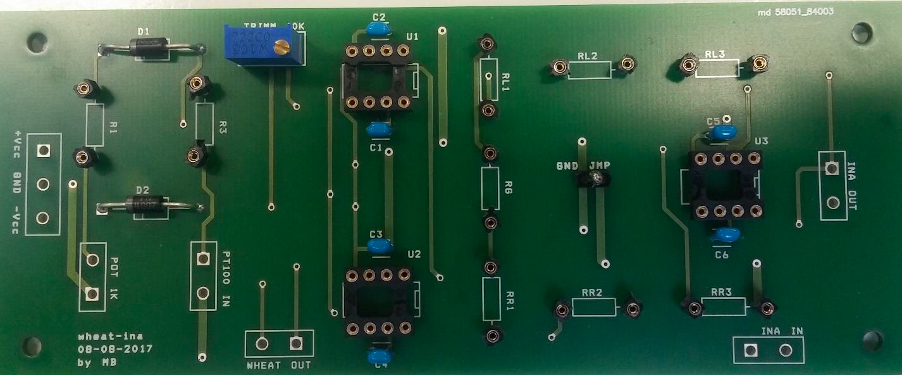
\includegraphics[width=\linewidth]{scheda_AMP_STRUM.png}
    \caption{Sopra: Schematico del ponte di Wheatstone e della configurazione utilizzata per effettuare misure. La tensione $+V_{cc}$ fornita al ponte è la stessa utilizzata per alimentare l'amplificatore per strumentazione. Sotto: fotografia del circuito integrato utilizzato. Questo contiene sia posto per le componenti dell'amplificatore per strumentazione, sia il ponte di Wheatstone.}
    \label{fig:circ_all}
\end{figure}

Vogliamo misurare la variazione di tensione ai capi del termometro al platino PT100, per ricavarne la resistenza interna che è legata in modo lineare alla variazione di temperatura. Poiché misuriamo variazioni di tensione possiamo decidere dove porre lo zero della misura, e perciò sfruttiamo il funzionamento del ponte di Wheatstone, che permette, in una precisa configurazione, di imporre il valore della tensione in uscita uguale a zero, e misurare solo le variazioni da questa condizione. Il ponte permette tale funzionamento solo se è ben bilanciato, ovvero se i prodotti incrociati delle resistenze sono uguali tra loro (nel caso della \reffig{fig:circ_all}: $R_1\cdot R_{PT}=R_2\cdot R_4$). Per evitare che la dissipazione di calore per effetto Joule possa influire sulla misura, impostiamo che la corrente massima che possa scorrere nel ramo del PT100 sia \SI{5}{\milli\ampere}. Poichè la tensione con cui alimentiamo il ponte è \SI{15}{\volt} in quanto utilizziamo $V_{cc}$, inserendo come $R_4$ una resistenza da \SI{3}{\kilo\ohm} e poichè questa resistenza è collegata in serie con il PT100 la resistenza complessiva dovrebbe essere \SI{3100}{\ohm} per cui la corrente nel ramo arriva a valere $V_{cc}/R_{tot}\approx\SI{5}{\milli\ampere}$. Imponendo la condizione per il bilanciamento del ponte e impostando il potenziometro a \SI{500}{\ohm} ricaviamo che $R_1$ deve valere \SI{15}{\kilo\ohm} 

Per controllare che il ponte sia effettivamente ben bilanciato, colleghiamo l'uscita del ponte all'oscilloscopio e regolando il potenziometro possiamo vedere quando il segnale è più vicino possibile a zero. Per fare una regolazione ancora migliore colleghiamo l'uscita del ponte all'amplificatore e quella dell'amplificatore all'oscilloscopio, in modo che pur essendo amplificato, il valore della tensione d'uscita, una volta regolata, sia comunque prossima a zero.

L'uscita del ponte di Wheatstone è collegata all'amplificatore per strumentazione in modo che la variazione di tensione sia amplificata e quindi misurabile in modo migliore. 


\section*{Presa dati}
Attraverso una interfaccia seriale e un programma di interpretazione del seriale possiamo acquisire e trascrivere a intervalli temporali regolari il valore di tensione misurato dal multimetro da banco Keitley che legge il segnale in uscita dall'amplificatore (\reffig{fig:circ_all}).

Lasciando il sistema allo stato iniziale (lampadina spenta e strumentazione di misura attiva) colleghiamo l'uscita dell'amplificatore all'oscilloscopio per osservare qualitativamente la dimensione della banda del rumore. 
Per quantificare tali fluttuazioni statistiche dovute al rumore utilizziamo il Keytley e acquisiamo per circa \SI{100}{\second} a intervalli regolari la misura della tensione. Una successiva analisi di questi dati ci porter\'a a quantificare l'errore per le successive misure.

Poiché vogliamo misurare l'andamento della temperatura rispetto alla distanza della sorgente posizioniamo tale sorgente a distanze fissate rispetto alla posizione del termometro PT100. Misurata tale distanza, vogliamo poi assicurarci che il termometro sia in una condizione stabile, e quindi avviamo il programma di acquisizione dati, e una volta che osserviamo valori stabili della tensione procediamo ad accendere la lampadina e da questo istante consideriamo un intervallo temporale tra i \SI{100}{\second} e \SI{180}{\second}, dopo il quale interrompiamo la presa dati. Ripetiamo questo processo per diversi  valori della distanza $d$.

\begin{figure*}
    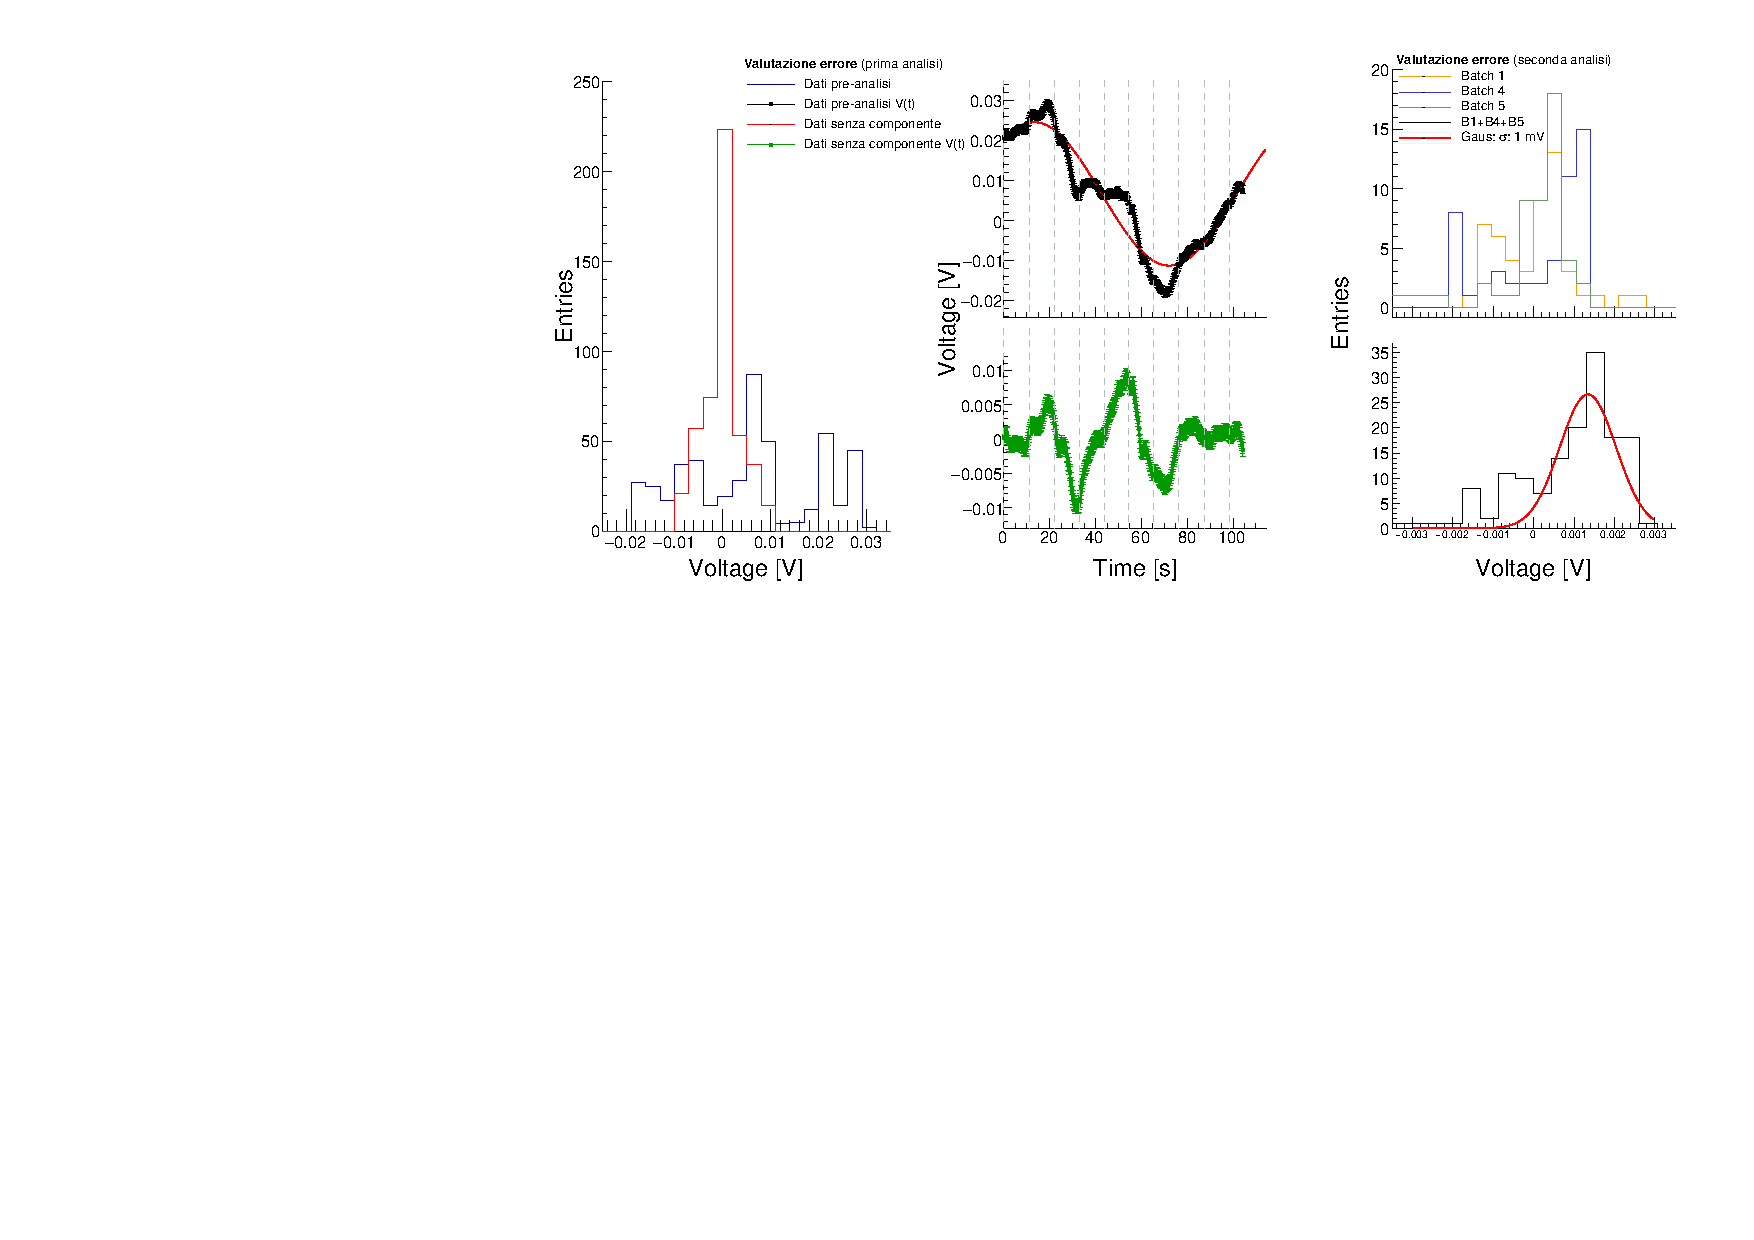
\includegraphics[width=\linewidth]{ErrVal2.pdf}
    \caption{Per la valutazione dell'errore abbiamo raccolto alcuni dati lasciando la strumentazione in tensione e la sorgente spenta. Questi dati, nel grafico in alto al centro (Dati pre-analisi V(t)) mostrano un comportamento riconducibile ad un segnale sinusoidale a bassa frequenza, e la relativa distribuzione, nell'istogramma (Dati pre-analisi), non è infatti riconducibile ad una curva gaussiana come atteso per una distribuzione di probabilità legata all'errore. In basso al centro (Dati senza componente V(t)) invece troviamo i dati trattati sottraendo la componente periodica sinusoidale, mostra un comportamento che non è imputabile alla presenza di altri componenti periodiche. Infatti la relativa distribuzione è ben più simile ad una distribuzione gaussiana, come osserviamo a sinistra in rosso. Questa componente però non può essere giustificata in nessun modo fisicamente, quindi ci preoccupiamo di dividere il segnale in batch di circa 50 punti di acquisizione l'uno e consideriamo quelli dove la curva non sembra oscillare periodicamente. Realizziamo dai batch 1, 4 e 5 quindi gli istogrammi (in alto a destra) e sommando i dati relativi a questi tre batch, osserviamo in un istogramma complessivo un comportamento che può essere gaussiano. Da quest'ultimo (in basso a destra) troviamo quindi il valore della deviazione standard ($1\sigma$) di \SI{1}{\milli\volt}.}
    \label{fig:errore}
\end{figure*}

\section*{Scelta dei dati raccolti}
Delle serie di dati raccolti effettuiamo una prima analisi di tipo qualitativo, semplicemente osservandone i grafici di tensione in funzione del tempo. Se il sistema si trova a riposo infatti la tensione in uscita non dovrebbe variare rispetto alla posizione iniziale se non per fluttuazioni legate all'ambiente e ad altri fattori casuali. Dovremmo quindi osservare un comportamento stabile fino all'istante in cui la lampadina non viene accesa cioè da quel momento in poi per cui la variazione di tensione è legata al fenomeno dell'irraggiamento. 

Prendiamo quindi in considerazione solo i dati per cui le fluttuazioni prima che la lampadina venga accesa siano almeno un ordine di grandezza inferiori alla variazione legata al fenomeno fisico considerato, ovvero per cui una volta accesa la lampadina, si osservi in modo evidente una variazione della tensione rispetto alla condizione di stabilità precedente. Decidiamo quindi di ignorare i valori presi per distanze maggiori di \SI{20}{\centi\metre}. Tuttavia  osserviamo che i dati raccolti a una distanza di \SI{15}{\centi\metre} non rientrano nelle condizioni prefissate, quindi non li consideriamo per successive analisi. 

Inoltre ci preoccupiamo di rimuovere i valori corrispondenti agli istanti precedenti all'accensione della lampadina, in quanto non sono influenti per la nostra analisi.

Infine procediamo ad analizzare i dati rimanenti eliminando eventuali errori di lettura dal seriale, ovvero punti facilmente individuabili dove per esempio due istatni di tempo successivi presentano la stessa lettura di tensione, o punti che presentano letture di tensione che non sono sensate rispetto alle grandezze misurate. 

\section*{Valutazione propagazione errori}

\noindent\textit{Errore sulla misura temporale---}
I punti sono acquisiti ad intervalli temporali regolari, controllati dal computer, che quindi possiamo considerare con un errore trascurabile rispetto alla misura effettuata, anche in relazione alle altre grandezze che entrano in gioco nella valutazione dell'errore complessivo sulla misura.

\noindent\textit{Errore sulla misura della tensione---}
Osservando i dati raccolti, rappresentanti le fluttuazioni legate al rumore o ad altri fenomeni di disturbo, notiamo un comportamento non totalmente imputabile a fluttuazioni casuali. Infatti è intuibile osservare la presenza di un segnale sinusoidale a frequenza molto bassa (vedi \reffig{fig:errore}). Per riuscire a sfruttare comunque questi dati decidiamo quindi di effettuare un fit secondo la funzione $p_0+p_1\cdot \cos(p_2\cdot (t-p_3))$ e sottraiamo questa funzione ai dati precedentemente raccolti ottenendo un comportamento in cui non è più possibile osservare componenti non casuali. Da questi nuovi dati possiamo quindi ricavare una distribuzione gaussiana dalla quale è possibile calcolare il valore della deviazione standard che utilizziamo come errore per i valori della tensione. Il valore ottenuto è pari a \SI{4.4}{\milli\volt}.

In realtà però un segnale che possiede una frequenza come quella della sinusoide che abbiamo ricavato (circa \SI{50}{\milli\hertz}), non è imputabile a nessun fenomeno fisico che conosciamo. Decidiamo quindi di procedere con una diversa analisi. Dividiamo i dati raccolti in 10 diversi batch da 50 punti ognuno e selezioniamo quelli in cui l'andamento della curva è più stabile, cioè i tratti più orizzontali. I batch che selezioniamo sono il primo, il quarto e il quinto. Da questi creiamo 3 diversi istogrammi e troviamo che il valore di RMS vale \SI{1}{\milli\volt} per ognuno. Centriamo i tre istogrammi in zero e successivamente sommiamo tutte le entrate per creare un unico istogramma (vedi \reffig{fig:errore}). Ricaviamo quindi il valore della deviazione standard che corrisponde all'errore sulla tensione che vale \[\varepsilon_{V} = \SI{1.0}{\milli\volt}.\]


\noindent\textit{Errore sulla misura della distanza---}
Per la misura di distanza entrano in gioco diversi fattori che influiscono sulla misura e che portano con sé un errore. La somma di tutti questi contributi, staticizzata, definisce quindi l'errore finale sulla misura ottenuta. 

\begin{table}
    \caption{Quantità e incertezze legate alla determinazione della distanza.}
    \label{tab:error:expected}
    \begin{ruledtabular}
        \begin{tabular}{ld}
            Quantità & \multicolumn{1}{c}{Incertezza} \\
            & \multicolumn{1}{c}{(\si{\milli\metre})} \\
            \colrule
            (stat) & \\
            \colrule
            % Allineamento del bulbo con il supporto & 1 \\
            Allineamento del supporto con il righello & 1 \\
            Allineamento del righello con la base del PT100 & 1 \\
            Errore di parallasse per ogni allineamento & 2 \\
            Errore sul possibile scivolamento durante le misure & 2 \\
            \colrule
            (syst) & \\
            \colrule
            Perpendicolarità degli indicatori di allineamento & \\
            sul PT100 & 3 \\
            Perpendicolarità degli indicatori di allineamento & \\
            sul supporto della lampada & 3 \\
            Disallineamento verticale/orizzontale sorgente/PT100\footnote{Non valutabile in una analisi dati a posteriori.} & \dots \\
            Totale statistico ($1\sigma$) & 6/\sqrt{3} \\
            Totale sistematico ($1\sigma$) & 6/\sqrt{3}
        \end{tabular}
    \end{ruledtabular}
\end{table}

\begin{figure*}
    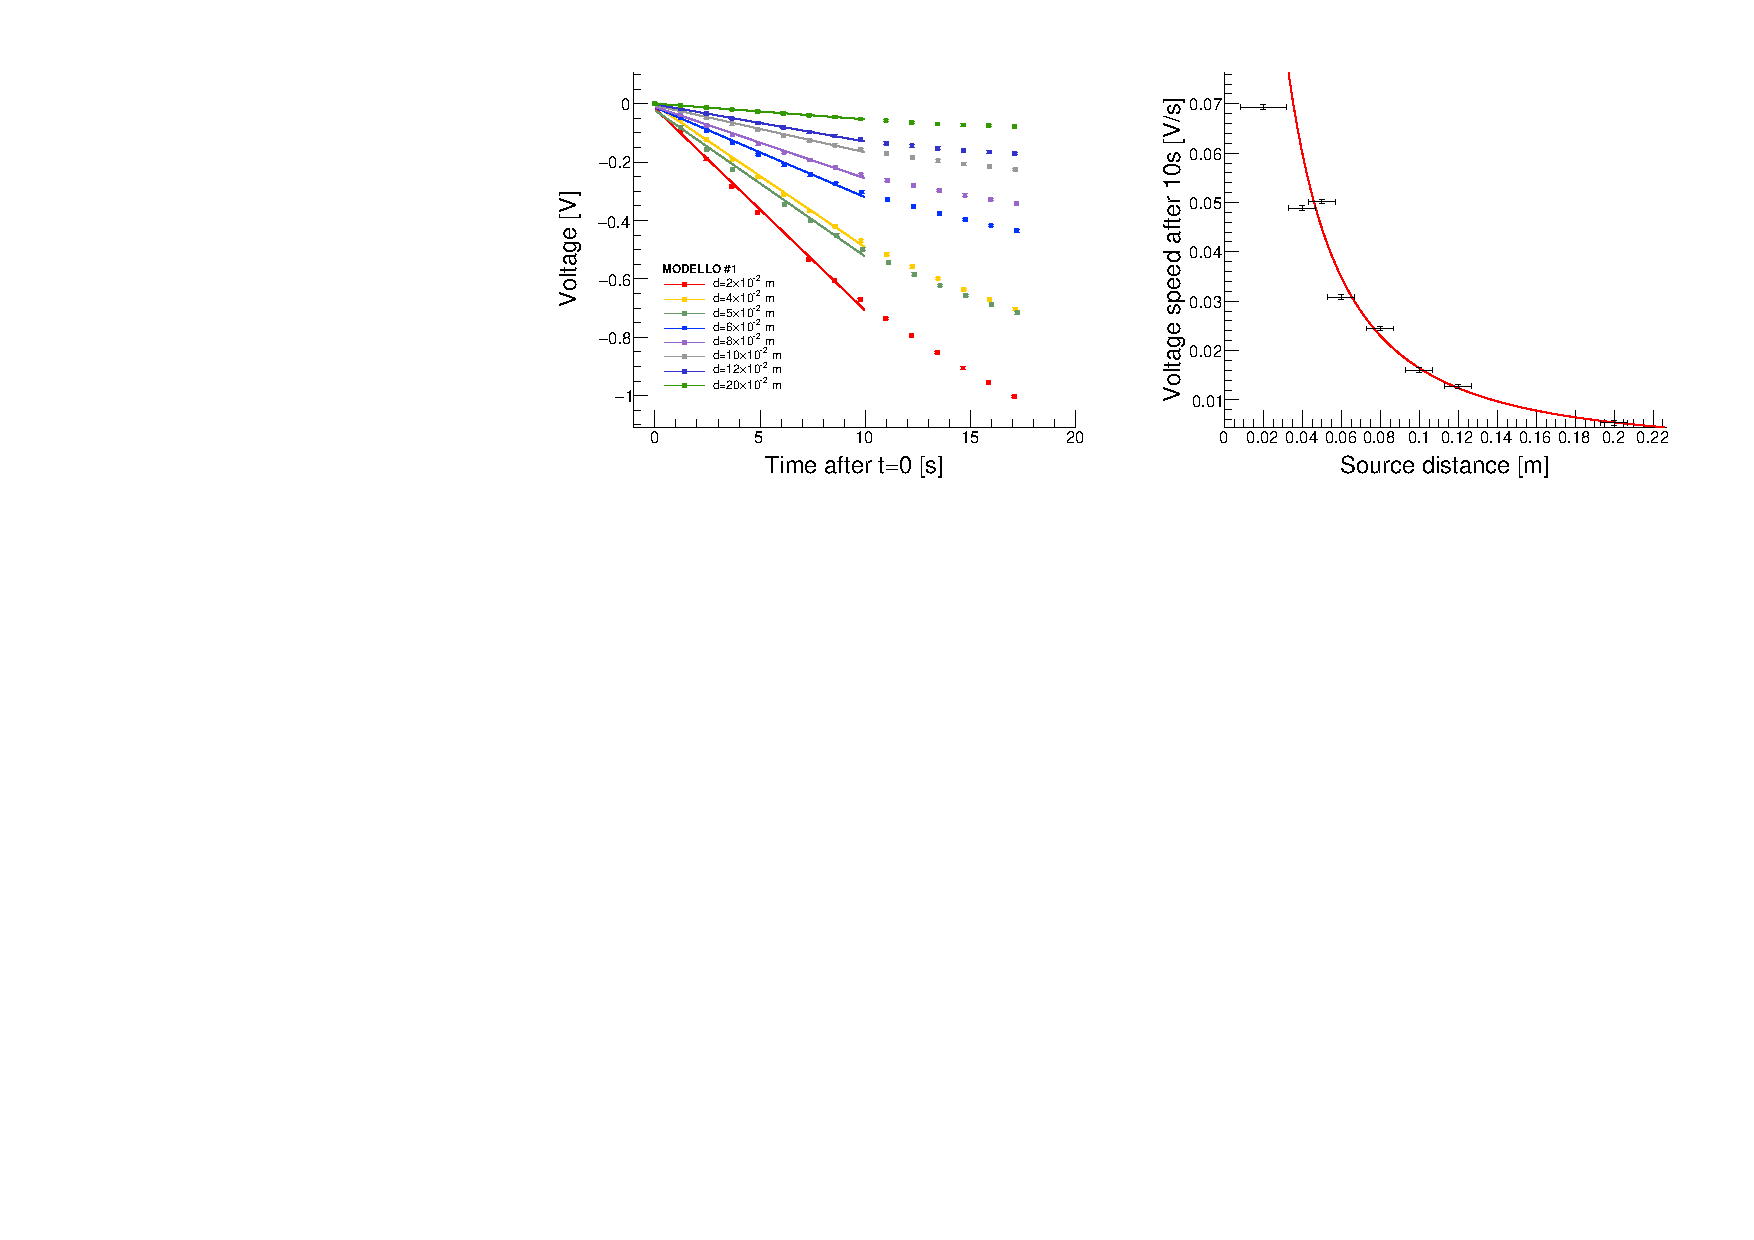
\includegraphics[width=\linewidth]{plot_mod1.pdf}
    \caption{\textbf{Applicazione del primo modello di analisi dei dati}. A sinistra abbiamo i diversi dati raccolti su cui eseguiamo un fit lineare entro un intervallo breve di tempo, ovvero fino a quando possiamo osservare il regime di linearità iniziale. Già visualmente si può osservare in questo modo che aumentando la distanza, la velocità con cui la tensione cambia non è sempre minore. Inoltre si possono già osservare anomalie su alcune distanze, come i dati a \SI{4}{\centi\metre} e \SI{5}{\centi\metre}, dove le due curve risultano invertite rispetto all'ordine crescente in cui si pongono le altre, anomalia che si ritrova anche nel grafico a destra. A destra invece troviamo più chiaro il comportamento $d^{a}$ come  previsto, anche se qualitativamente non è facile individuare il range in cui $a$ può trovarsi.}
    \label{fig:plot:mod1}
\end{figure*}

In \reftab{tab:error:expected} abbiamo riportato le possibili fonti di errore. Consideriamo \SI{1}{\milli\metre} come errore di allineamento, ovvero l'accuratezza dello strumento in uso, e poiché l'allineamento lo effettuiamo sia dalla parte del sensore che dalla parte della sorgente, questa incertezza la consideriamo due volte. Inoltre poiché questa misura viene effettuata manualmente è anche soggetta ad un possibile errore di parallasse sulla misura, che valutiamo di \SI{1}{\milli\metre} per ogni allineamento, quindi \SI{2}{\milli\metre} in totale. Otteniamo un totale statistico di $6/\sqrt{3}$ mm.

Oltre all'errore statistico possiamo individuare una serie di errori sistematici che possono essere presenti. In primo luogo l'allineamento della sorgente e del PT100 con il righello era effettuato sfruttando un segno a matita che individuava un punto sulla base dei due strumenti. Però Questi segni potrebbero non essere precisi e soffrire di un disallineamento con lo strumento stesso (il PT100 o il centro della lampadina), che abbiamo stimato comunque poter essere al più \SI{3}{\milli\metre} ciascuna. 

Infine è probabile che sorgente e sensore non siano posti in asse, quindi presentino un offset orizzontale e verticale, per cui la distanza reale $d_{\text{r}}$ è maggiore alla distanza misurata $d_{\text{meas}}$, in quanto 
\[
    d_{\text{r}} = \sqrt{d_{\text{meas ($x$)}}^2 + \delta_y^2 + \delta_z^2}.
\]
Questi valori però non sono stati raccolti in laboratorio, per cui non siamo in grado di fornire una stima. Inoltre l'effetto di questo disallineamento diviene più evidente più la distanza $d_{\text{meas}}$ tra sorgente e sensore diventa piccola.


\begin{figure*}
    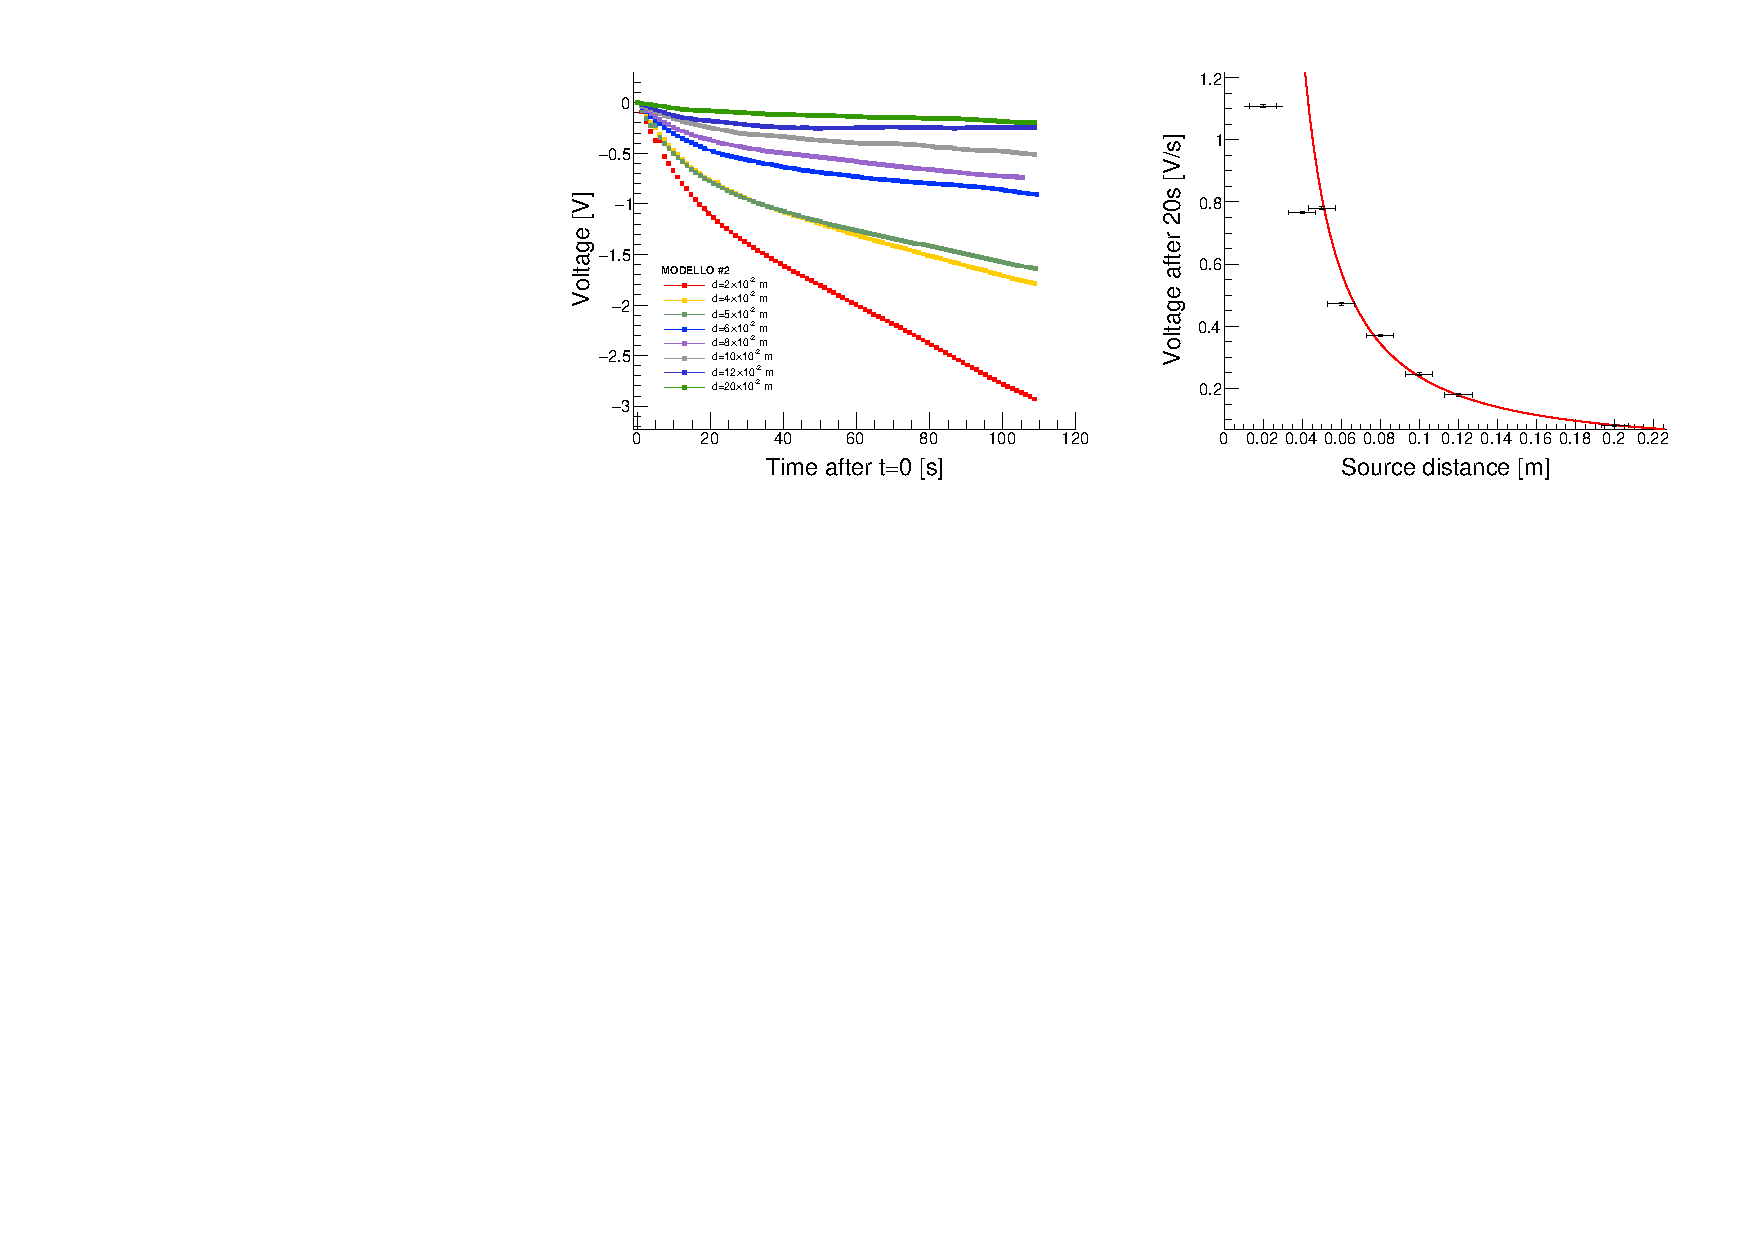
\includegraphics[width=\linewidth]{plot_mod2.pdf}
    \caption{\textbf{Applicazione del secondo modello di analisi dei dati}. A sinistra abbiamo i diversi dati raccolti su cui eseguiamo un fit lineare entro un intorno del punto che vogliamo misurare, per poter effettuare una misura ad una data distanza temporale, poiché i dati non si presentano continui. Si può inoltre osservare come di fatto dopo circa \SI[parse-numbers=false]{30/40}{\second} il comportamento della tensione diventi lineare, in accordo con quanto ipotizzato possa essere il suo comportamento pratico. A destra invece troviamo più chiaro il comportamento $d^{a}$ come  previsto, anche se qualitativamente non è facile individuare il range in cui $a$ può trovarsi. L'errore è quello valutato a seguito di una analisi sulle incertezze sistematiche, la banda orizzontale segna questa incertezza complessiva, i marker verticali indicano dove era stimato l'errore precedente a queste considerazioni. Questo cambiamento è ben visibile sopratutto nel primo punto.}
    \label{fig:plot:mod2}
\end{figure*}

\section*{Modello \#1 di analisi della variazione di tensione}
I dati ottenuti si presentano come letture di tensione in funzione del tempo. Non essendo a conoscenza di una precisa legge fisica che regoli questo andamento della tensione in relazione al tempo, possiamo però procedere ipotizzando alcuni modelli che possano descrivere il fenomeno che si osserva. 

Innanzitutto quando la lampadina viene accesa la luce raggiunge in modo immediato il sensore resistivo che quindi, per il fenomeno dell'irraggiamento, viene scaldato, e poiché la resistenza del PT100 dipende in modo lineare dalla sua temperatura, cambierà anche la tensione ai capi dello strumento. Tuttavia la lampadina scalda anche il vetro e l'aria che circondano il nostro sensore. Questo trasferimento di calore al vetro e all'aria fa sì che il PT100 risenta anche del loro effetto. Noi però siamo interessati solamente all'effetto prodotto dalla lampadina per mezzo dell'irraggiamento. Poiché quindi possiamo considerare la velocità di trasferimento di calore per irraggiamento molto maggiore della velocità di trasferimento di calore per conduzione termica, ipotizziamo che i primi secondi dall'accensione della lampadina siano caratterizzati principalmente dall'effetto dell'irraggiamento. 

Inoltre, ad un primo ordine di approssimazione su $t$, per i primi secondi possiamo ipotizzare che l'andamento della tensione sia lineare. Osservando i dati raccolti vediamo che il massimo intervallo che possiamo prendere affinché il comportamento lineare della curva sia presente in tutti i grafici che abbiamo selezionato è di \SI{10}{\second} per tutte le curve (si veda \reffig{fig:plot:mod1}). 

Eseguendo un fit lineare possiamo quindi ottenere il valore della velocità di variazione della tensione $dV/dt$ per ogni distanza che abbiamo selezionato.

A questo punto procediamo a raccogliere le coppie $(d,~dV/dt)$ in un grafico per poterne osservare il comportamento. La nostra ipotesi è infatti che maggiore è la distanza, minore sarà la velocità con cui la tensione cambierà a causa dell'irraggiamento. 

Vogliamo infatti verificare che i punti raccolti siano in relazione come 
\[
    \frac{dV}{dt} \propto d^{-2}
\]
e quindi eseguiamo un fit come
\begin{equation}\label{eq:modello_plot}
    \frac{dV}{dt} = p_0\cdot(d+p_2)^{a}
\end{equation}
per cui vogliamo verificare che il fattore $a$ sia compatibile con il valore atteso di $a = -2$, mentre il valore di $p_2$ rappresenta l'eventuale offset sui valori raccolti della distanza. Il parametro $p_0$ rappresenta invece la costante di proporzionalità, ed è caratteristica del problema che stiamo considerando.


\section*{Modello \#2 di analisi della variazione di tensione}

\begin{figure}
    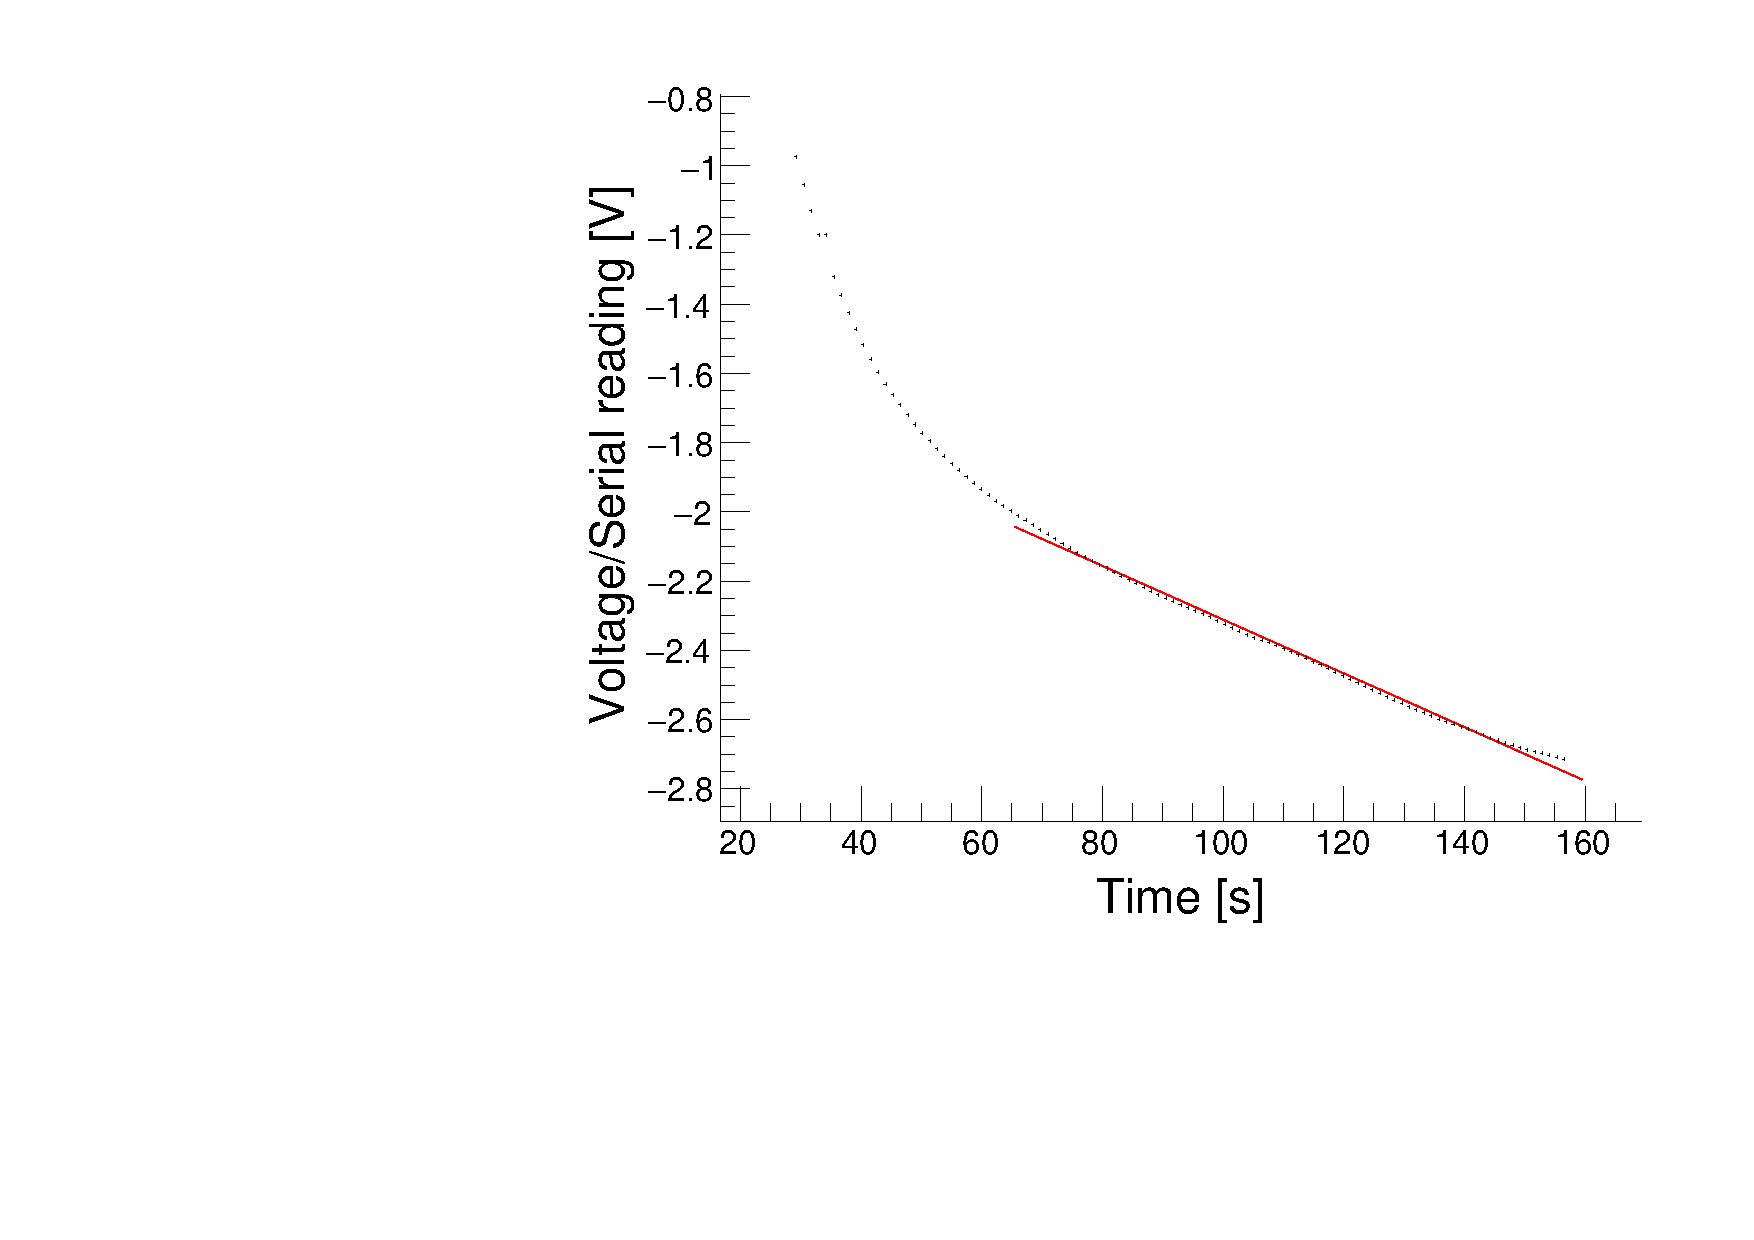
\includegraphics[width=\linewidth]{LinTest.pdf}
    \caption{Evidenziamo come in effetti si possa eseguire un fit lineare su una curva dei dati (per esempio è stata presa la curva ottenuta ad una distanza di \SI{5e-2}{\metre}) dopo un iniziale intervallo di tempo dove presupponiamo invervenga principalmente un fattore legato all'irraggiamento. }
    \label{fig:plot:linear}
\end{figure}

Invece che limitarci a considerare la variazione dei valori entro i primi punti dove il comportamento è prettamente lineare, andiamo ora a considerare la variazione di tensione su intervalli temporali più estesi, dove non possiamo però conoscere con certezza il modello fisico-matematico che sta dietro al fenomeno. Perciò, invece che calcolare la velocità di variazione, consideriamo un intervallo fisso di tempo $\Delta t_1$ (scegliamo per esempio \SI{20}{\second}), dopo il quale, una volta posto il valore della tensione a zero all'istante iniziale ($t=0$), vogliamo valutare la variazione della d.d.p. Il problema principale che si pone è che i dati raccolti sono dati discreti e probabilmente non presentano una lettura della tensione esattamente dopo $\Delta t_1$ s; quindi, poichè il grafico in un primo ordine di approssimazione per il tempo per un intervallo sufficientemente piccolo può essere approssimato come $p_0+x\cdot p_1$, possiamo eseguire dei fit localizzati in un intorno [$\Delta t_1-2$ s; $\Delta t_1+2$ s] e poi estrapolare il valore di tensione in un istante preciso. Procedendo poi come già fatto per il Modello \#1, possiamo eseguire un fit in base all'equazione equazione \ref{eq:modello_plot} e andiamo a verificare la compatibilità del parametro $p_1$ con -2.

Proviamo infine a considerare intervalli diversi, e per ognuno di questi $\Delta t$ ripetiamo lo stesso procedimento. Possiamo quindi vedere qual è il massimo valore di $\Delta t $ che ci permette di trovare la compatibilità del parametro $p_1$ con -2 per capire effettivamente se e quando diventa rilevante il contributo degli altri fattori diversi dall'irraggiamento.

\section*{risultati e conclusioni}

\begin{figure}
    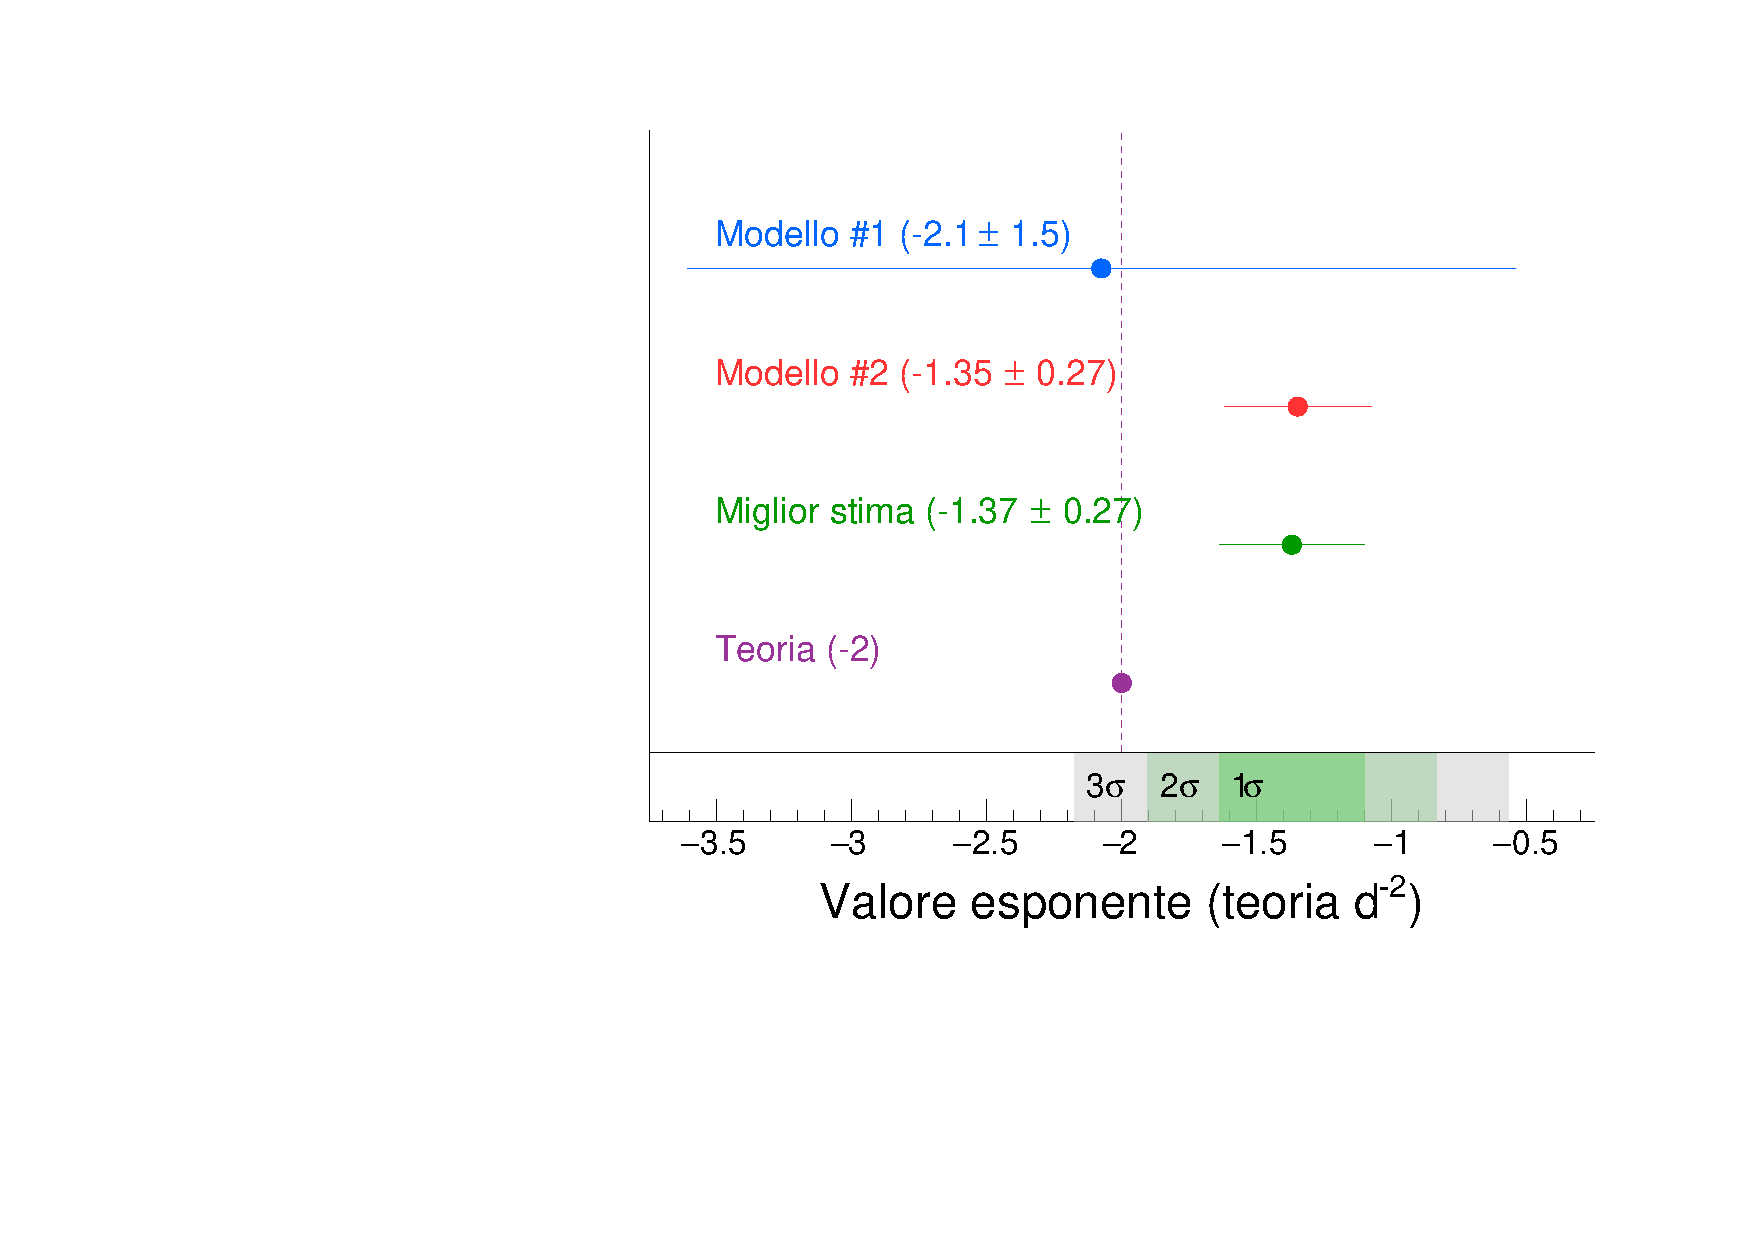
\includegraphics[width=\linewidth]{results.pdf}
    \caption{Risultati dell'esperienza rispetto al modello \#1 e \#2, con miglior stima ricavata dai risultati compatibili dei due modelli, che presenta significatività statistica rispetto alla teoria di $2.8\sigma$.}
    \label{fig:results}
\end{figure}


Dal Modello \#1 otteniamo che per ogni distanza che abbiamo selezionato l'approssimazione lineare al primo ordine funziona e otteniamo quindi 8 coppie di valori $(d,~dV/dt)$ che già visivamente mostrano un andamento compatibile con la teoria. Realizzando quindi il fit, per il quale il valore di \ChiNdf~è 3.9/5 con $P(\chi^2)=55.8\%$, il valore dell'esponente $a$ ottenuto dall'esperimento è \[a\text{(mod-1)}=\num{-2.07574 +- 1.53327}\] mentre il valore dell'offset lungo la distanza è pari a \SI[round-mode=none]{4 +- 11}{\centi\metre}. Perciò considerando la compatibilità entro $3\sigma$ verifichiamo che il valore dell'esponente è compatibile con quanto previsto dalla teoria e che anche il valore dell'offset è compatibile con zero. Questa compatibilità dell'offset con zero è dovuta alla presenza di un errore molto elevato che però non siamo in grado di spiegare in quanto è legato al modo in cui il programma fa i calcoli per il fit.

La prima analisi realizzata secondo il modello \#2 è stata fatta con $\Delta t=20s$. Questo valore lo abbiamo scelto perchè nella maggior parte delle distanze selezionate rappresentava l'inizio di un secondo regime lineare dovuto ad altri fenomeni diversi dall'irraggiamento (\reffig{fig:plot:linear}). Dal fit, per cui abbiamo \ChiNdf~ 2.3/5 con $P(\chi^2)=80.7\%$, otteniamo che il valore dell'esponente risulta essere \[a\text{(mod-2)}=\num{-1.32084 +- 0.16688}\] e quindi non compatibile con -2 con la significatività statistica pari a $4.1\sigma$. Di conseguenza c'è molta probabilità che gli intervalli di tempo maggiori di 20s non daranno compatibilità e infatti, verificandolo, abbiamo osservato un comportamento analogo. Abbiamo quindi provato con dei $\Delta t$ minori. Tuttavia anche in questi casi non troviamo compatibilità. Possiamo quindi dire che il modello \#2 non è valido per descrivere il fenomeno che abbiamo analizzato. In realtà abbiamo notato che se si aumenta di pochi millimetri (circa \num{2.9}) l'errore sulla distanza del punto relativo a $d=\SI{2}{\centi\metre}$, che è la distanza per cui l'effetto del disassamento diventa più evidente, allora la compatibilità è presente fino a circa $\Delta t=\SI{30}{\second}$. Perciò, se ammettiamo di aver sottostimato l'errore preso qui in considerazione, allora il modello \#2 diventa valido e compatibile con la teoria e inoltre mostra, come effettivamente ci aspettavamo, che dopo un certo tempo il fenomeno in analisi cambia ed è quindi necessario cambiare modello. In questo secondo caso otterremmo come valore \[a'\text{(mod-2)}=\num{-1.34804 +- 0.272111}\] con \ChiNdf~ 2.3/5 e con $P(\chi^2)=81.1\%$. 

Poiché i due risultati sono tra loro compatibili può essere sensato calcolare la miglior stima (Exp) ottenuta da $a\text{(mod-1)}$ e $a'\text{(mod-2)}$ del valore di $a$ \[a\text{(Exp)} = \num{-1.37026 +- 0.267924}\] che risulta essere compatibile anch'essa con $-2$ entro $2.4\sigma$. Visualizziamo infine i risultati in figura \ref{fig:results}.



\begin{methods}{D\lowercase{ati completi e codice sorgente}}
    Tutti i dati completi a supporto dei grafici, e il relativo codice, sono visualizzabili su \url{https://github.com/mattiasotgia/Lab2}. L'analisi dati viene eseguita su un programma sviluppato in C++ basandosi su framework pubblici: ROOT, per la realizzazione dei grafici e il fit dei modelli (\url{https://root.cern/}).
\end{methods}

%\onecolumngrid
\appendix

% \setcounter{table}{0}
\renewcommand{\thetable}{S-\arabic{table}}
\renewcommand{\thefigure}{S-\arabic{figure}}
\begin{figure}[p]
    \raggedright
    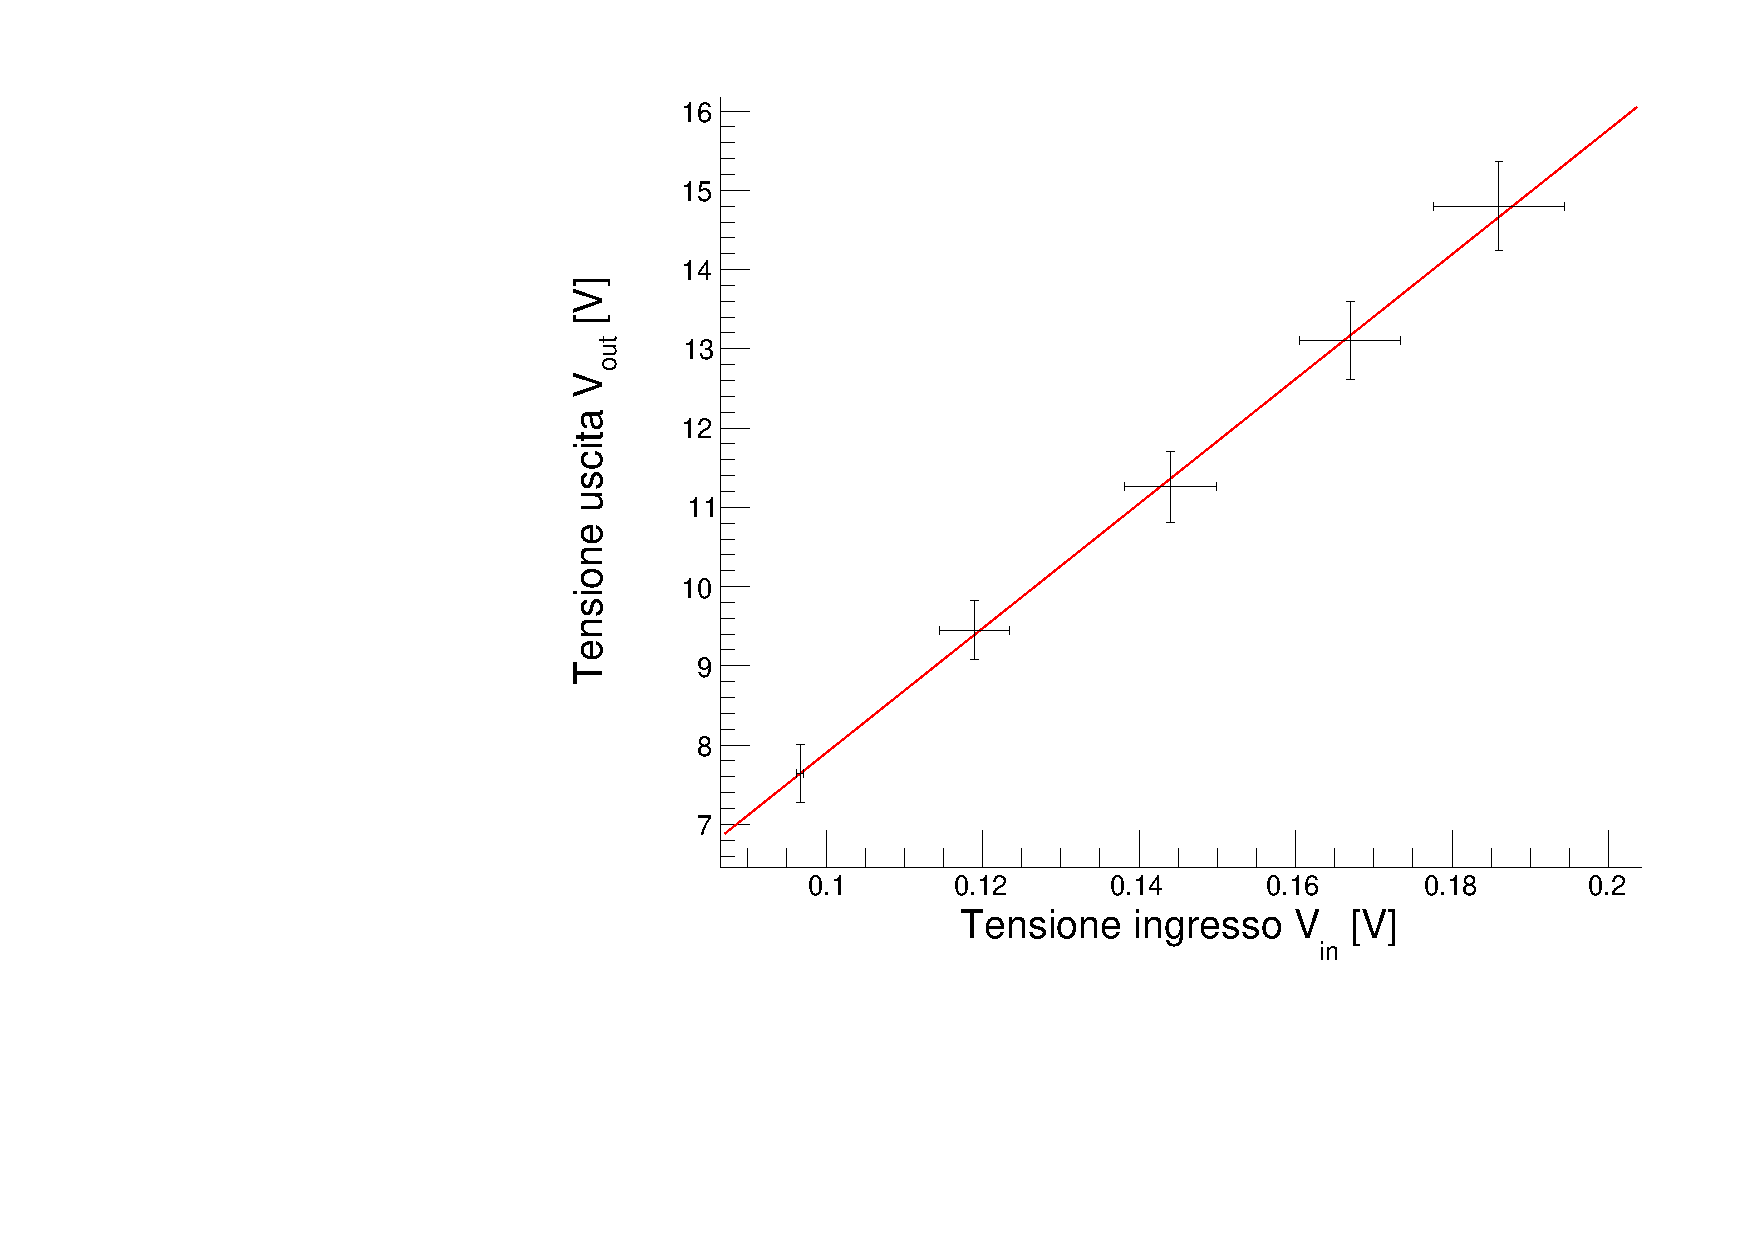
\includegraphics[width=\linewidth]{Guadagno__invertente.pdf}
    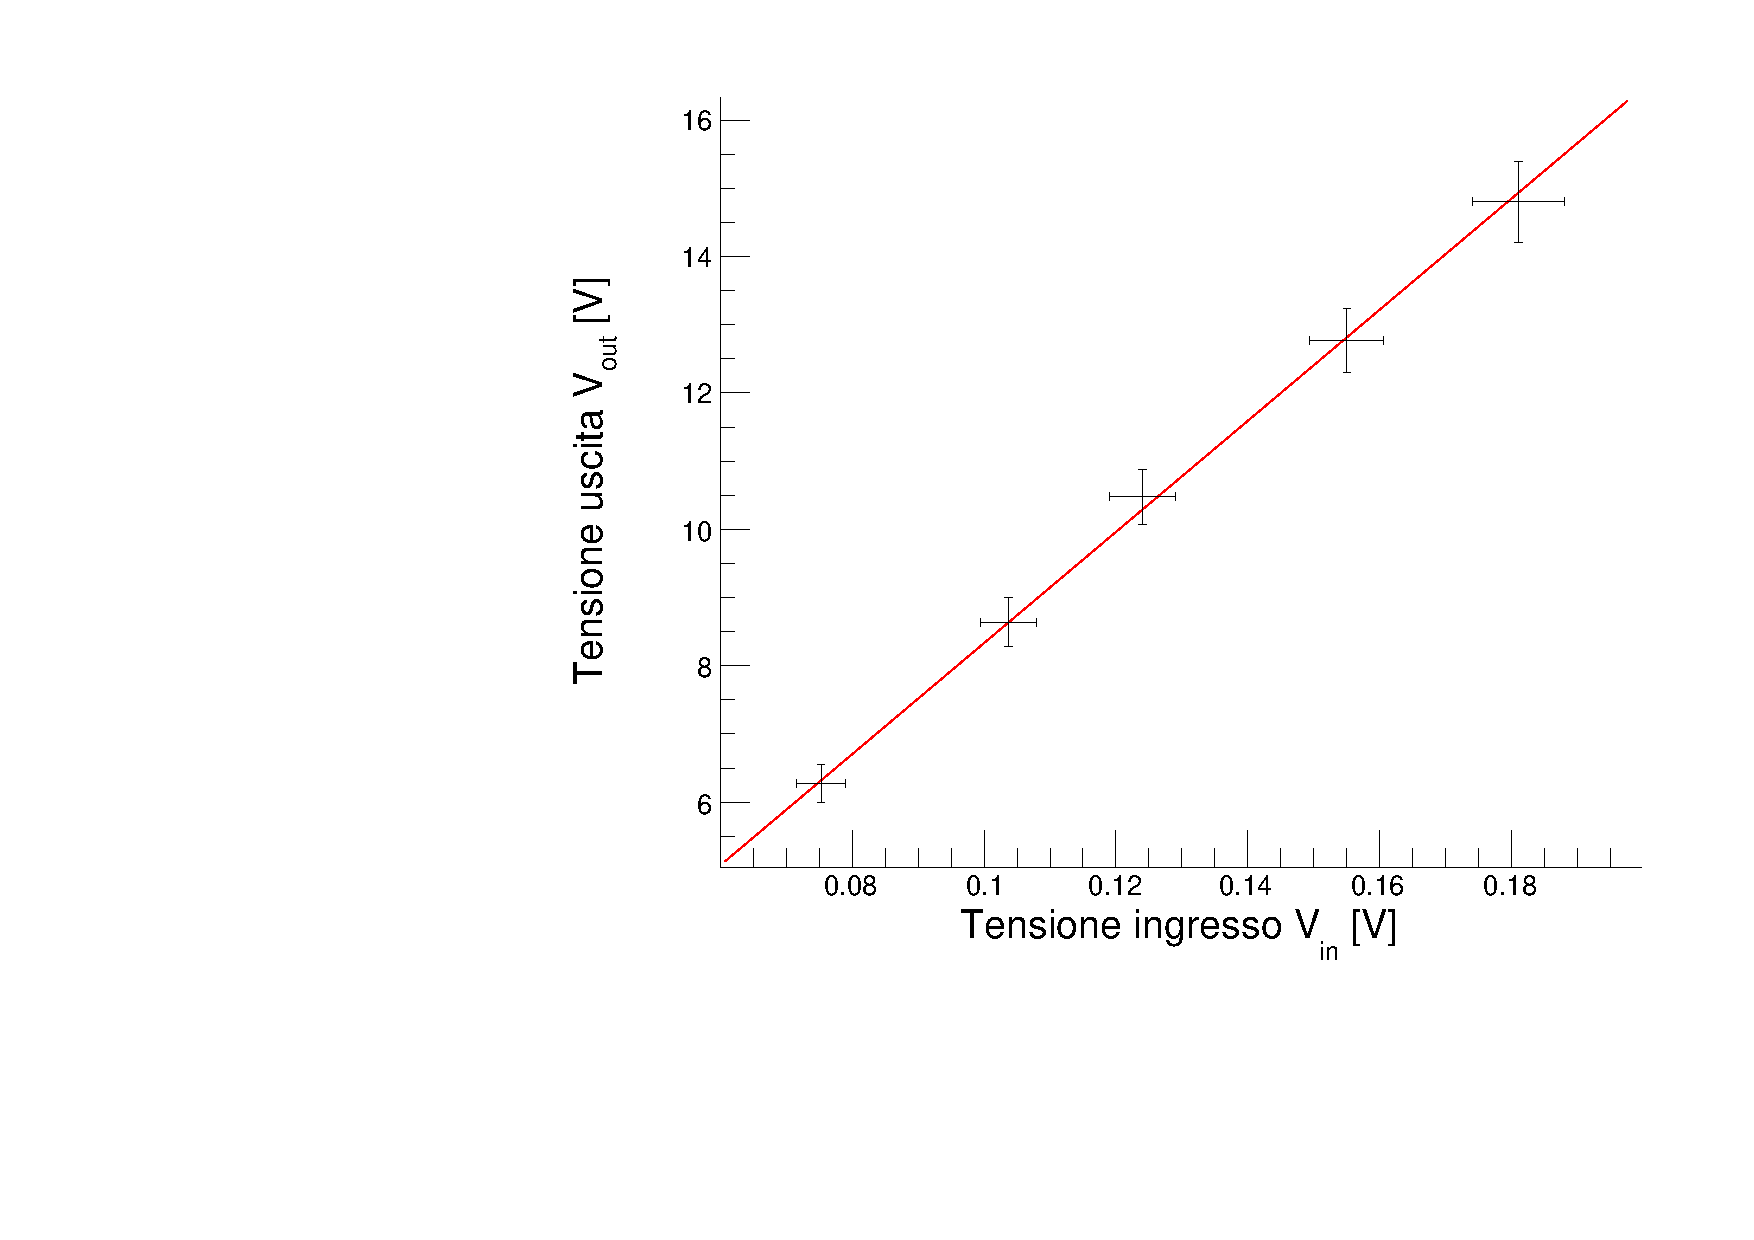
\includegraphics[width=\linewidth]{Guadagno__noninvertente.pdf}
    \caption{\textbf{Misura del guadagno degli amplificatori operazionali realizzati in sezione \ref{sec:studio_caratt_op_amp}.} Sopra: valori variabili di tensione in ingressso e in uscita per misurare il guadagno dello strumento, in configurazione invertente. Sotto: come sopra, per la configurazione non invertente.}
    \label{fig:guadagno_inv_noninv}
\end{figure}
\begin{figure}[p]
    \raggedright
    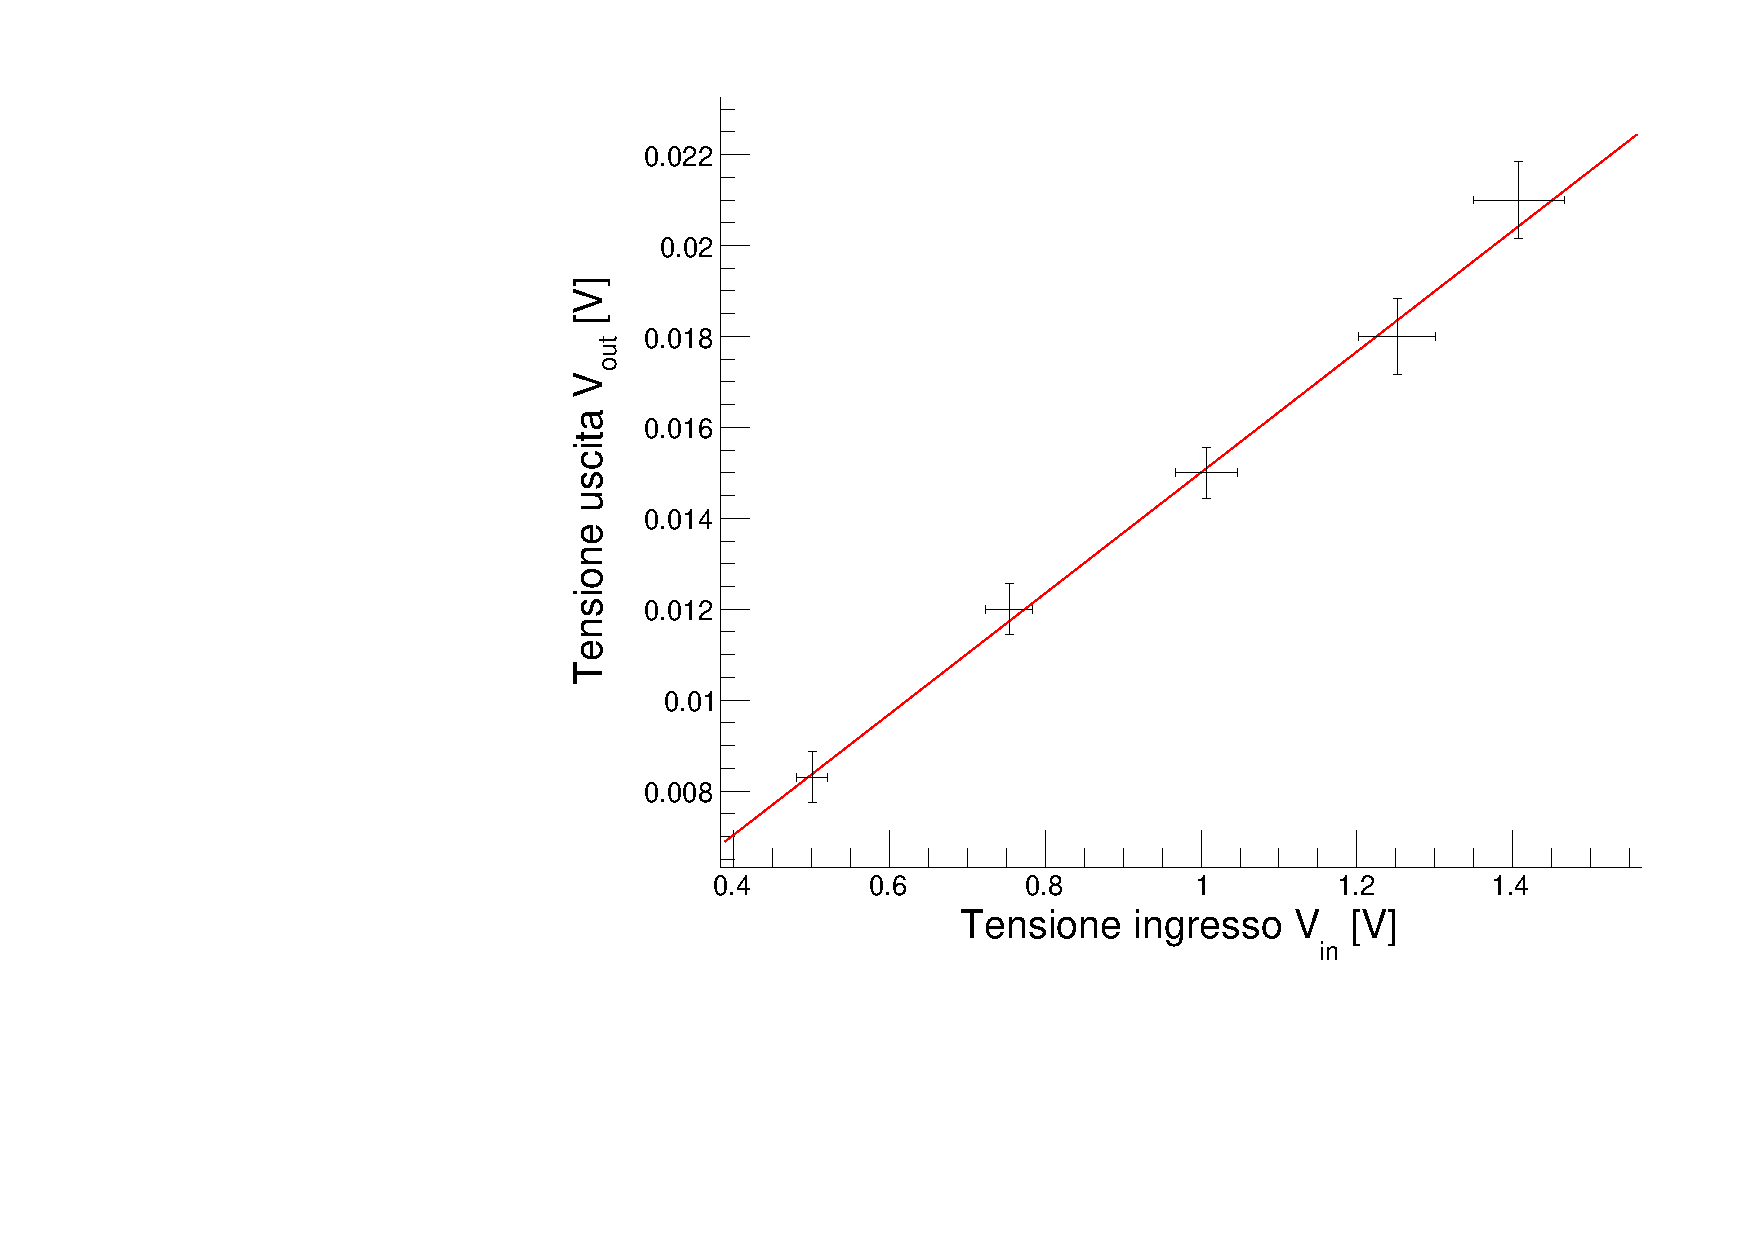
\includegraphics[width=\linewidth]{GuadagnoMC.pdf}
    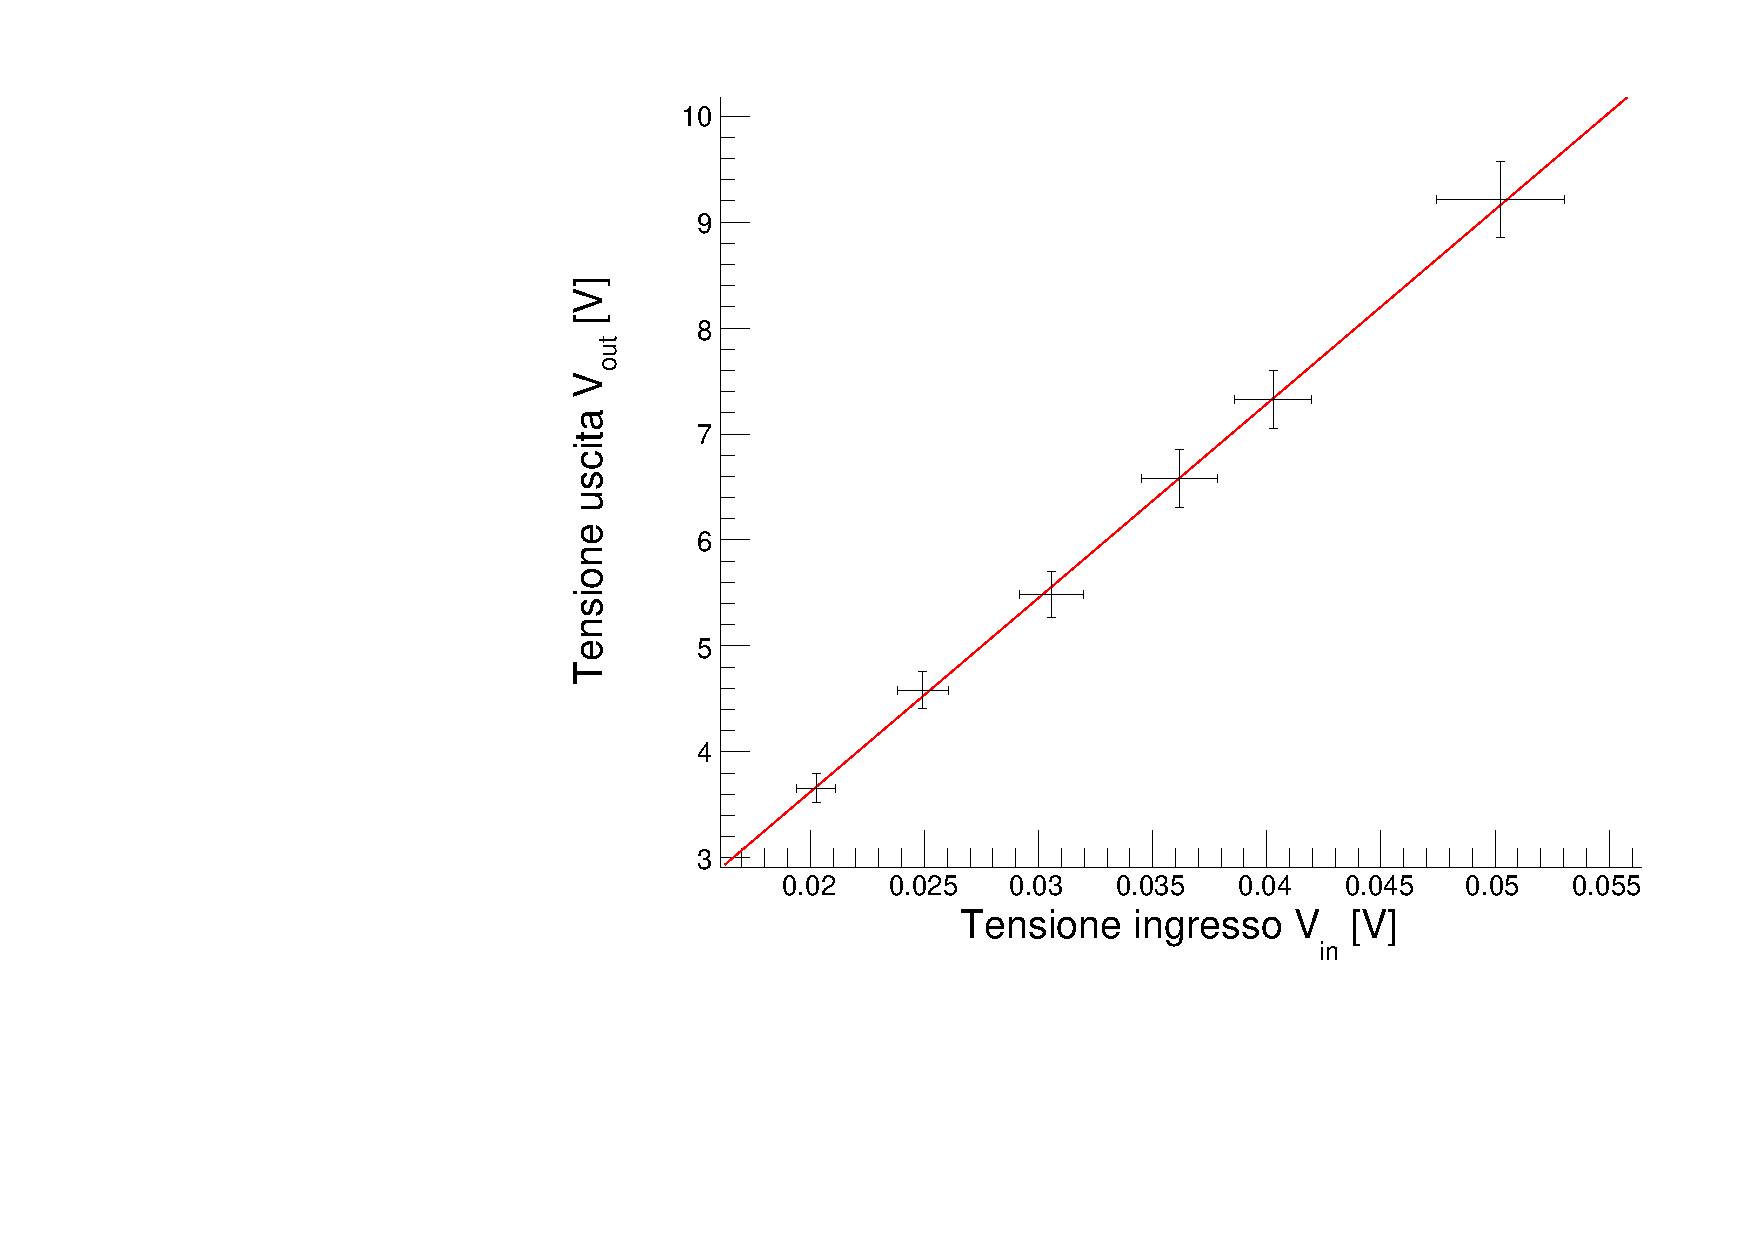
\includegraphics[width=\linewidth]{GuadagnoDIFF.pdf}
    \caption{\textbf{Analisi del guadagno dell'amplificatore per strumentazione.} Sopra: Analisi del guadagno in modo comune $G_{\text{CM}}$ dell'amplificatore per strumentazione ottenute misurando la tensione in ingresso e in uscita all'amplificatore operazionale, fornendo tensione uguale al capo invertente e non invertente. Sotto: Analisi del guadagno differenziale $G_{\text{diff}}$ dell'amplificatore per strumentazione, eseguito utilizzando tensioni diverse ai capi invertente e non invertente.}
    \label{fig:guadagno_op_amp_strum}
\end{figure}

\end{document}
    
